\chapter[Menyelesaikan Program Linier secara Grafis]{Menyelesaikan Program Linier secara Grafis\texorpdfstring{\protect\footnotemark}{}}
\footnotetext{Sebagian bab ini diadaptasi dari materi \emph{A First Course in Linear Programming} karya Kevin Cheung (Carleton University), yang dilisensikan dengan CC BY-SA 4.0, dengan modifikasi oleh Robert Hildebrand. Lihat bab Sumber dan Atribusi untuk perinciannya.}

\begin{outcome}
\begin{enumerate}
\item[A.] Gambarkan daerah titik yang diperbolehkan oleh kendala, beserta garis aras fungsi objektif.
\item[B.] Tentukan titik-titik sudut daerah tersebut dan hitung koordinatnya.
\item[C.] Baca solusi optimal langsung dari gambar.
\item[D.] Kenali empat kemungkinan hasil program linier: satu titik terbaik, satu sisi penuh yang terdiri atas titik-titik terbaik, sama sekali tidak ada titik yang diperbolehkan, atau nilai objektif yang meningkat tanpa batas.
\end{enumerate}
\end{outcome}
\begin{resource}
\begin{itemize}
\item \href{https://www.youtube.com/watch?v=K7TL5NMlKIk&ab_channel=Dr.TreforBazett}{YouTube! -- Pemodelan dengan Program Linier -- Tonton 4:20 -- Selesai}
\item \href{https://www.youtube.com/watch?v=E72DWgKP_1Y&t=1014s&ab_channel=TomS}{YouTube! -- Tonton 1:43 -- 3:43}
\end{itemize}
\end{resource}

\begin{tryit}
\vizlink{objective-slider}{Penggeser Aras Objektif}: geser garis objektif melintasi daerah layak dan amati tempat optimum tercapai.
\end{tryit}


Program linier dengan dua variabel keputusan dapat digambarkan seluruhnya pada selembar kertas: setiap kendala memotong bidang dengan sebuah garis, titik-titik yang lolos dari setiap pemotongan membentuk daerah layak, dan fungsi objektif menjadi keluarga garis sejajar, satu untuk setiap nilai objektif yang mungkin. Dengan menggeser sebuah garis dari keluarga ini melintasi daerah tersebut dan mengamati tempat garis itu keluar, kita memperoleh cara yang sepenuhnya visual untuk menemukan titik terbaik. Gambaran inilah yang menjadi pokok bahasan bab ini.

Kita mulai dengan contoh kecil yang berperilaku baik dan mudah digambar. Setelah geometrinya dipahami, kita beralih ke contoh-contoh dengan persoalan yang memberikan pelajaran penting.

%% Gambar hiasan program linier dihapus (berkas tidak tersedia)

\section{Masalah Tak Kosong dan Terbatas}\label{sec:nonempty-bounded}

Perhatikan masalah berikut:
\begin{align*}
\max \quad & 2 x_1+5 x_2 \\
\text { dengan syarat } \quad
&x_1+2 x_2 \leq 16 \\
&5 x_1+3 x_2 \leq  45 \\
&x_1, x_2  \geq 0
\end{align*}

Langkah pertama adalah menggambar \emph{daerah layak}: semua titik $(x_1, x_2)$ yang memenuhi seluruh kendala sekaligus.

Cara yang andal untuk menggambarnya ialah memulai dari batas: gambar garis tempat setiap kendala berlaku sebagai persamaan, yaitu
\begin{itemize}
\item $x_1+2 x_2 = 16$
\item $5 x_1+3 x_2 = 45$
\item $x_1 = 0$
\item $x_2= 0$
\end{itemize}
kemudian arsir sisi bidang yang ditentukan oleh pertidaksamaan terkait.

\begin{figure}[h!]
\begin{center}
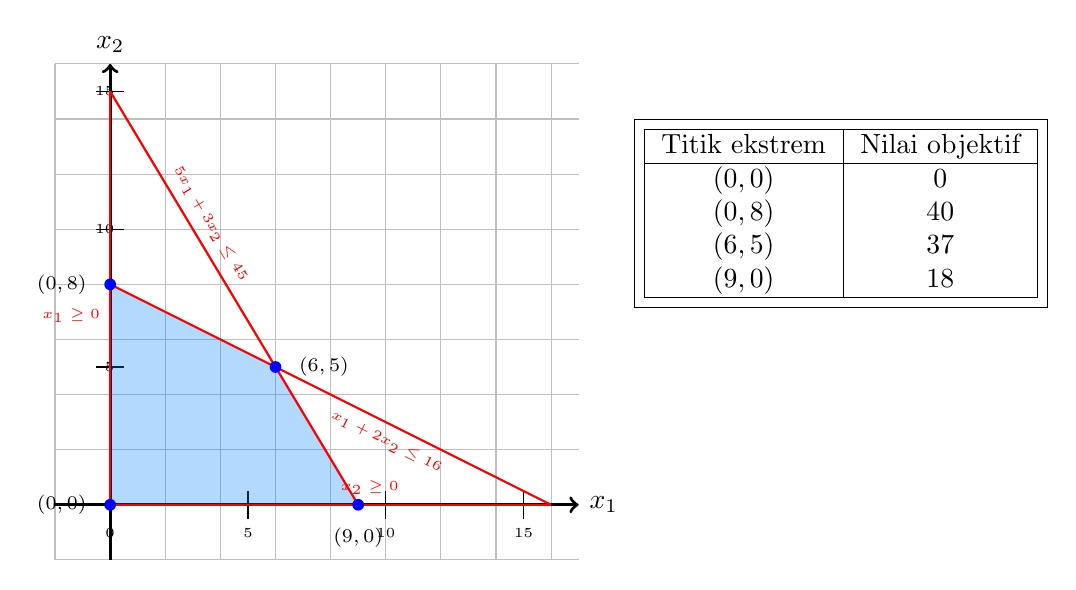
\begin{tikzpicture}[scale = 0.35]
    % Kisi dan sumbu
    \draw[gray!50, thin, step=2] (-2,-2) grid (17,16);
    \draw[very thick,->] (-2,0) -- (17,0) node[right] {$x_1$};
    \draw[very thick,->] (0,-2) -- (0,16) node[above] {$x_2$};

    % Label sumbu
    \foreach \x in {0,5,10,15} \draw (\x,0.5) -- (\x,-0.5) node[below] {\tiny\x};
    \foreach \y in {0,5,10,15} \draw (-0.5,\y) -- (0.5,\y) node[left] {\tiny\y};

    % Daerah layak yang diarsir
    \fill[blue!50!cyan,opacity=0.3] (0,0) -- (0,8) -- (6,5) -- (9,0) -- cycle;

    % Garis kendala
    \draw[red,thick] (0,8) -- node[below right,sloped] {\tiny$x_1 + 2x_2 \leq 16$} (16,0);
    \draw[red,thick] (0,15) -- node[above left,sloped] {\tiny$5x_1 + 3x_2 \leq 45$} (9,0);
    \draw[red,thick] (0,0) -- node[below left] {\tiny$x_1 \geq 0$} (0,15);
    \draw[red,thick] (0,0) -- node[above right] {\tiny$x_2 \geq 0$} (16,0);

    % Titik ekstrem
    \node[blue] at (0,0) [circle,fill,inner sep=1.5pt]{};
    \node[blue] at (0,8) [circle,fill,inner sep=1.5pt]{};
    \node[blue] at (6,5) [circle,fill,inner sep=1.5pt]{};
    \node[blue] at (9,0) [circle,fill,inner sep=1.5pt]{};

    % Label titik ekstrem
    \node[black,anchor=east] at (-0.5,0) {\scriptsize$(0,0)$};
    \node[black,anchor=east] at (-0.5,8) {\scriptsize$(0,8)$};
    \node[black,anchor=west] at (6.5,5) {\scriptsize$(6,5)$};
    \node[black,anchor=north] at (9,-0.5) {\scriptsize$(9,0)$};
% Tabel di dalam gambar TikZ
    \node[draw,fill=white,anchor=north west] at (19,14) {
        \begin{tabular}{|c|c|}
        \hline
        Titik ekstrem & Nilai objektif \\
        \hline
        $(0,0)$ & $0$ \\
        $(0,8)$ & $40$ \\
        $(6,5)$ & $37$ \\
        $(9,0)$ & $18$ \\
        \hline
        \end{tabular}
    };
\end{tikzpicture}
\end{center}
\caption{\href{https://www.desmos.com/calculator/j1li4l7lcv}{Desmos: grafik interaktif!} (\href{https://open-optimization.github.io/open-optimization-or-book/interactive-figures/lp-graphical-method.html}{grafik interaktif cadangan})}
\end{figure}

Setiap garis membagi bidang menjadi dua; dengan mempertahankan sisi yang benar dari setiap garis dan mengarsir bagian yang bertahan, kita memperoleh daerah layak.

Ada dua sifat daerah ini yang perlu diberi nama. Daerah ini \emph{tak kosong}: sekurang-kurangnya satu titik memenuhi setiap kendala. Daerah ini juga \emph{terbatas}: seluruh daerah dapat dimuat di dalam suatu lingkaran besar dan tidak memanjang selamanya ke arah mana pun.

Sudut-sudut daerah, yang disebut \emph{titik ekstrem}, ternyata memuat semua informasi yang kita perlukan mengenai solusi optimal. Setiap sudut terletak pada perpotongan dua garis batas, sehingga koordinat sudut diperoleh dengan menyelesaikan sistem linier $2 \times 2$. Namun, berhati-hatilah: perpotongan dua garis batas merupakan syarat perlu, tetapi bukan syarat cukup, sebab dua garis juga dapat berpotongan pada titik yang melanggar kendala ketiga.

Kelak kita akan menggunakan istilah \emph{solusi basis layak} untuk titik ekstrem daerah layak, dan \emph{solusi dasar} untuk titik perpotongan 2 garis yang ternyata tak layak (tidak memenuhi semua kendala).

\begin{theorem}{Solusi Optimal pada Titik Ekstrem}\label{thm:optimalextremepoint}
Jika daerah layak suatu program linier tak kosong dan terbatas, maka terdapat solusi optimal pada sebuah titik ekstrem daerah layak tersebut.
\end{theorem}

Teorema ini menyiratkan algoritma berikut.
\begin{algorithm}[H]
\caption{Algoritma Enumerasi Titik Ekstrem untuk Menyelesaikan Masalah Program Linier}
\label{alg:EnumerateVertices}
\begin{enumerate}
    \item \textbf{Tentukan Daerah Layak:}
    Tentukan himpunan kendala yang mendefinisikan daerah layak dalam masalah tersebut.
    \item \textbf{Enumerasikan Titik Ekstrem:}
    Temukan semua titik ekstrem (titik sudut) daerah layak. Caranya ialah menyelesaikan pasangan-pasangan persamaan kendala untuk mencari perpotongannya, lalu hanya mempertahankan titik yang memenuhi semua kendala.
    \item \textbf{Hitung Nilai Objektif:}
    Evaluasi fungsi objektif pada setiap titik ekstrem daerah layak.
    \item \textbf{Bandingkan Nilai Objektif:}
    Untuk masalah maksimisasi, tentukan titik ekstrem dengan nilai objektif tertinggi. Untuk masalah minimisasi, tentukan titik ekstrem dengan nilai objektif terendah.
    \item \textbf{Tentukan Solusi Optimal:}
    Titik ekstrem dengan nilai objektif optimal adalah solusi masalah program linier tersebut.
\end{enumerate}
\end{algorithm}

Kita akan mempelajari alasan Teorema~\ref{thm:optimalextremepoint} berlaku, serta apa yang terjadi ketika daerah layak tidak memenuhi asumsi tak kosong ataupun terbatas.

\section{Pendekatan Grafis}\label{sec:graphical-approach}
Sekarang kita menerapkan gagasan enumerasi titik ekstrem secara grafis dengan sebuah contoh konkret.

\begin{example}{Bengkel Mebel}\label{ex:FurnitureWorkshop}
Sebuah bengkel mebel kecil memproduksi kursi dan meja. Setiap kursi memerlukan 2 jam pengerjaan kayu dan 1 jam penyelesaian akhir serta menghasilkan laba \$8. Setiap meja memerlukan 1 jam pengerjaan kayu dan 3 jam penyelesaian akhir serta menghasilkan laba \$6. Bengkel tersebut memiliki 80 jam waktu pengerjaan kayu dan 90 jam waktu penyelesaian akhir per minggu. Permintaan pasar membatasi produksi kursi hingga paling banyak 32 buah per minggu.

Misalkan $x_1$ menyatakan jumlah kursi dan $x_2$ menyatakan jumlah meja. Program liniernya adalah:
\begin{equation}
\begin{aligned}
\max\;\;& z(x_1,x_2) = 8x_1 + 6x_2\\
\text{dengan syarat}\;\;&  2x_1 + x_2 \leq 80\\
& x_1 + 3x_2 \leq 90\\
& x_1 \leq 32\\
& x_1 \geq 0\\
& x_2 \geq 0
\end{aligned}
\label{eqn:FurnitureWorkshop}
\end{equation}
\end{example}

\begin{solution} Untuk menyelesaikannya secara grafis, mula-mula kita menggambar daerah layak dengan memplot garis batas setiap kendala dan mengarsir daerah yang memenuhi semua pertidaksamaan secara bersamaan. Hasilnya ditunjukkan pada Gambar~\ref{fig:FurnitureWorkshopFeasibleRegion}.

\begin{figure}[H]
\centering
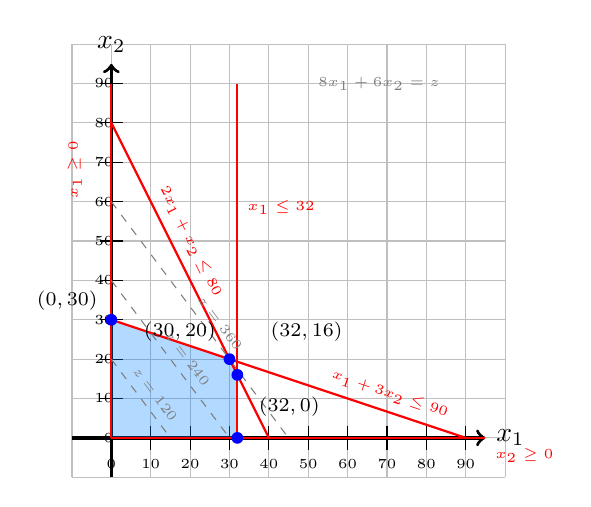
\begin{tikzpicture}[scale=0.05]
    % Kisi dan sumbu
    \draw[gray!50, thin, step=10] (-10,-10) grid (100,100);
    \draw[very thick,->] (-10,0) -- (95,0) node[right] {$x_1$};
    \draw[very thick,->] (0,-10) -- (0,95) node[above] {$x_2$};

    % Label sumbu
    \foreach \x in {0,10,...,90} \draw (\x,3) -- (\x,-3) node[below] {\tiny\x};
    \foreach \y in {0,10,...,90} \draw (-3,\y) -- (3,\y) node[left] {\tiny\y};

    % Titik ekstrem daerah layak: (0,0), (0,30), (30,20), (32,16), (32,0)
    \fill[blue!50!cyan,opacity=0.3]
        (0,0) -- (0,30) -- (30,20) -- (32,16) -- (32,0) -- cycle;

    % Garis kendala
    \draw[red,thick] (0,80) --  node[pos=0.20,above right,sloped] {\tiny $2x_1 + x_2 \leq 80$}(40,0);
    \draw[red,thick] (0,30) --  node[pos=0.58,above right,sloped] {\tiny $x_1 + 3x_2 \leq 90$}(90,0);
    \draw[red,thick] (32,90) --  node[pos=0.35,right] {\tiny $x_1 \leq 32$}(32,0);
    \draw[red,thick] (0,0) -- (95,0) node[below right] {\tiny $x_2 \geq 0$};
    \draw[red,thick] (0,0) -- (0,90);
    \node[red,rotate=90,anchor=south] at (-5,68) {\tiny $x_1 \geq 0$};

    % Kurva aras fungsi objektif (8x1 + 6x2 = z)
    \draw[dashed,gray] (0,120/6) -- node[pos=0.55,above,sloped] {\tiny $z = 120$} (120/8,0);
    \draw[dashed,gray] (0,240/6) -- node[pos=0.55,above,sloped] {\tiny $z = 240$} (240/8,0);
    \draw[dashed,gray] (0,360/6) -- node[pos=0.55,above,sloped] {\tiny $z = 360$} (360/8,0);

    % Label titik ekstrem
    \node[blue] at (0,30) [circle,fill,inner sep=1.5pt]{};
    \node[blue] at (30,20) [circle,fill,inner sep=1.5pt]{};
    \node[blue] at (32,16) [circle,fill,inner sep=1.5pt]{};
    \node[blue] at (32,0) [circle,fill,inner sep=1.5pt]{};

    % Koordinat titik ekstrem
    \node[black,anchor=south east] at (-1,30) {\scriptsize $(0,30)$};
    \node[black,anchor=south east] at (29,22) {\scriptsize $(30,20)$};
    \node[black,anchor=south west] at (38,22) {\scriptsize $(32,16)$};
    \node[black,anchor=south west] at (35,3) {\scriptsize $(32,0)$};

    % Label fungsi objektif
    \node[gray] at (68,90) {\tiny $8x_1 + 6x_2 = z$};
\end{tikzpicture}
\caption{Daerah layak dan kurva aras untuk masalah Bengkel Mebel. Poligon berarsir menyatakan himpunan semua $(x_1,x_2)$ yang memenuhi setiap kendala. Garis putus-putus menunjukkan fungsi objektif pada beberapa nilai $z$. Ketika $z$ meningkat, kurva aras bergeser ke atas dan ke kanan.}
\label{fig:FurnitureWorkshopFeasibleRegion}
\end{figure}

Berikutnya, kita menumpangkan kurva aras fungsi objektif. Dengan menetapkan $8x_1 + 6x_2 = z$, diperoleh keluarga garis
\[
x_2 = -\tfrac{4}{3}\,x_1 + \tfrac{z}{6},
\]
yang merupakan garis-garis sejajar dengan kemiringan $-4/3$. Peningkatan $z$ menggesernya ke arah gradien $\nabla z = (8,6)$. Dengan menyapukan kurva aras ke arah ini, kurva terakhir yang menyentuh daerah layak menyentuh titik ekstrem $(x_1^*,x_2^*) = (30,20)$, sehingga menghasilkan laba optimal
\[
z^* = 8(30) + 6(20) = 360.
\]

Titik optimal ini berada pada perpotongan dua kendala $2x_1+x_2=80$ dan $x_1+3x_2=90$. Kedua kendala dipenuhi sebagai persamaan pada optimum; kita menyebutnya \textit{aktif}. Kendala-kendala lainnya ($x_1\leq 32$, $x_1\geq 0$, $x_2\geq 0$) dipenuhi secara ketat dan disebut \textit{tidak aktif}.

Hal ini menggambarkan prinsip umum: ketika solusi optimal suatu program linier ada, solusi tersebut terjadi pada titik ekstrem daerah layak, yakni perpotongan beberapa kendala aktif.
\end{solution}

Sekarang kita dapat menyatakan algoritma awal untuk menyelesaikan program linier dua variabel dengan daerah layak terbatas secara grafis.
\begin{stepbox}{algpivot}{\ding{192}\ Metode Grafis 1: Daerah Terbatas, Optimum Tunggal}
\begin{enumerate}[nosep]
\item Gambar daerah layak dengan memplot batas setiap kendala dan mengarsir perpotongan semua setengah bidang.
\item Gambar beberapa kurva aras fungsi objektif $z = c_1 x_1 + c_2 x_2$ untuk nilai $z$ yang makin besar.
\item Sapukan kurva aras ke arah gradien $\nabla z = (c_1, c_2)$ hingga ditemukan kurva aras terakhir yang masih menyentuh daerah layak.
\item Titik ekstrem daerah layak yang terletak pada kurva aras terakhir ini adalah solusi optimal.
\end{enumerate}
\end{stepbox}

\begin{example}{Pedagang Limun}\label{exa:lemonadevendor}
Misalkan Anda menjual limun dan sari lemon. Setiap unit limun
memerlukan 1 buah lemon dan 2 liter air. Setiap unit sari lemon
memerlukan 3 buah lemon dan 1 liter air. Setiap unit limun menghasilkan
laba tiga dolar. Setiap unit sari lemon menghasilkan laba dua
dolar. Anda memiliki 6 buah lemon dan 4 liter air. Berapa unit
limun dan sari lemon yang sebaiknya dibuat untuk memaksimumkan laba?

Jika \(x\) menyatakan jumlah unit limun yang akan dibuat dan
\(y\) menyatakan jumlah unit sari lemon yang akan dibuat, maka
laba dalam dolar diberikan oleh \(3x + 2y\). Kita menyebut \(3x + 2y\)
sebagai fungsi objektif. Perhatikan bahwa terdapat sejumlah kendala yang
harus dipenuhi oleh \(x\) dan \(y\). Pertama, \(x\) dan \(y\) harus
tak negatif. Jumlah lemon yang diperlukan untuk membuat \(x\) unit limun
dan \(y\) unit sari lemon adalah \(x+3y\) dan tidak boleh melebihi 6.
Jumlah liter air yang diperlukan untuk membuat \(x\) unit limun dan
\(y\) unit sari lemon adalah \(2x+y\) dan tidak boleh melebihi 4. Jadi,
untuk menentukan laba maksimum, kita perlu memaksimumkan \(3x + 2y\)
dengan syarat \(x\) dan \(y\) memenuhi kendala \(x + 3y \leq 6\),
\(2x + y \leq 4\), \(x \geq 0\), dan \(y \geq 0.\)

Cara yang lebih ringkas untuk menuliskan masalah ini adalah sebagai berikut:
\[\begin{array}{rrcrll}
\text{maksimumkan } & 3x & + & 2y & \\
\text{dengan syarat}
& x & + & 3y & \leq & 6 \\
& 2x & +&  y & \leq & 4 \\
& x &  & & \geq & 0 \\
& & & y & \geq & 0. \\
\end{array}\]

\end{example}
\begin{solution}
Kita dapat menyelesaikan masalah maksimisasi ini secara grafis sebagai
berikut. Mula-mula kita menggambar himpunan $(x,y)$ yang memenuhi
semua kendala, yang disebut daerah layak, pada bidang \((x,y)\). Kemudian
kita mengubah fungsi objektif \(3x+2y\) menjadi persamaan garis
\(3x+2y = z\), dengan \(z\) sebagai parameter. Ketika nilai \(z\)
meningkat, garis yang didefinisikan oleh persamaan \(3x+2y=z\) bergerak
ke arah vektor normal
$(3,2)$. Arah ini kita sebut
arah perbaikan. Menentukan nilai maksimum fungsi objektif,
yang disebut nilai optimal, dengan tetap memenuhi kendala setara dengan
mencari nilai maksimum \(z\) sedemikian sehingga garis yang didefinisikan
oleh persamaan \(3x+2y=z\) masih berpotongan dengan daerah layak.

\begin{figure}[H]
\centering
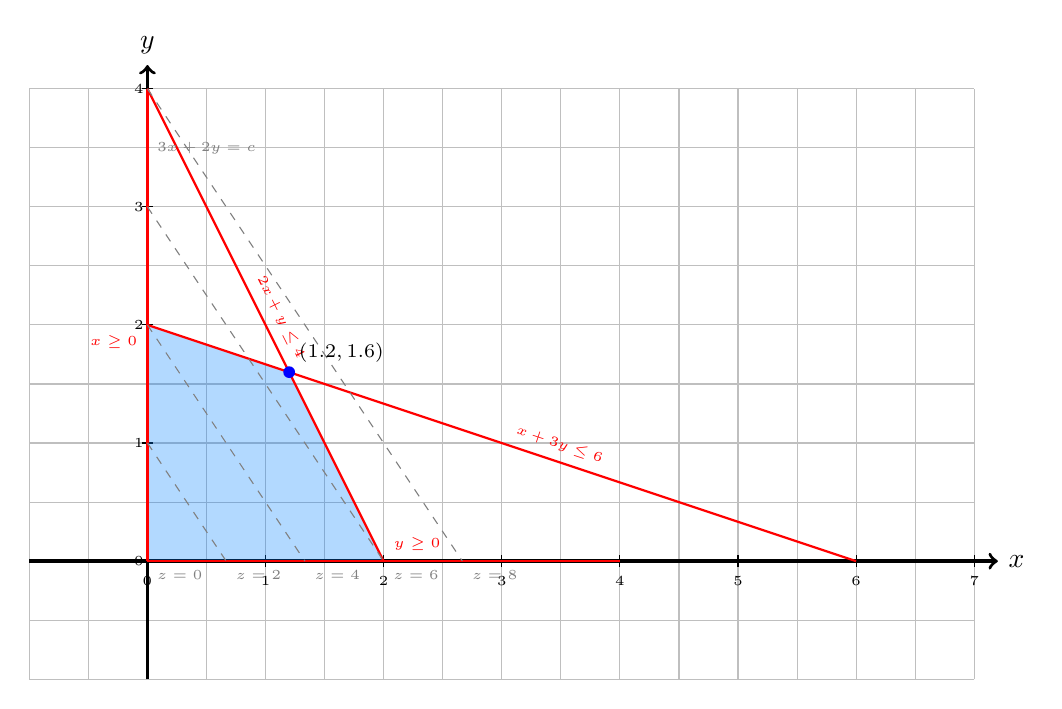
\begin{tikzpicture}[scale = 1.5]
    % Kisi dan sumbu
    \draw[gray!50, thin, step=0.5] (-1,-1) grid (7,4);
    \draw[very thick,->] (-1,0) -- (7.2,0) node[right] {$x$};
    \draw[very thick,->] (0,-1) -- (0,4.2) node[above] {$y$};

    % Label sumbu
    \foreach \x in {0,...,7} \draw (\x,0.05) -- (\x,-0.05) node[below] {\tiny\x};
    \foreach \y in {0,...,4} \draw (-0.05,\y) -- (0.05,\y) node[left] {\tiny\y};

    % Daerah layak yang diarsir
    \fill[blue!50!cyan,opacity=0.3] (0,0) -- (0,2) -- (1.2,1.6) -- (2,0) -- cycle;

    % Garis kendala
    \draw[red,thick] (0,2) -- node[above right,sloped] {\tiny$x + 3y \leq 6$} (6,0);
    \draw[red,thick] (0,4) -- node[above,sloped] {\tiny$2x + y \leq 4$} (2,0);
    \draw[red,thick] (0,0) -- node[below left] {\tiny$x \geq 0$} (0,4);
    \draw[red,thick] (0,0) -- node[above right] {\tiny$y \geq 0$} (4,0);

        % Kurva aras fungsi objektif
            \draw[dashed,gray] (0,4) -- (8/3,0) node[below right] {\tiny$z=8$};
    \draw[dashed,gray] (0,3) -- (2,0) node[below right] {\tiny$z=6$};
    \draw[dashed,gray] (0,2) -- (4/3,0) node[below right] {\tiny$z=4$};
    \draw[dashed,gray] (0,1) -- (2/3,0) node[below right] {\tiny$z=2$};
    \draw[dashed,gray] (0,0) -- (0,0) node[below right] {\tiny$z=0$};

    % Label kontur
    \node[gray] at (0.5,3.5) {\tiny$3x + 2y = c$};

     \node[blue] at (1.2,1.6) [circle,fill,inner sep=1.5pt]{};

    % Label titik ekstrem
    \node[black,anchor=south west] at (1.2,1.6) {\scriptsize$(1.2,1.6)$};
\end{tikzpicture}
\caption{Daerah layak dan kurva aras objektif untuk masalah Pedagang Limun. Poligon berarsir adalah himpunan $(x,y)$ yang memenuhi semua kendala; garis putus-putus merupakan kurva aras $3x+2y = z$ untuk $z = 0,2,4,6,8$. Penyapuan kurva aras ke arah $\nabla z = (3,2)$ menunjukkan bahwa optimum berada pada titik ekstrem $(1.2,1.6)$.}
\label{fig:LemonadeVendorFeasibleRegion}
\end{figure}

% TODO: TikZ pinjaman dari Stack Exchange di bawah menampilkan program linier 3 kendala yang tidak terkait
% (x_1+x_2>=3, 2x_1-x_2<=5, -x_1+2x_2<=3) dan tampak tidak pada tempatnya dalam
% solusi Pedagang Limun. Tidak ditemukan padanan hasil reka ulang; dipertahankan
% sambil menunggu tinjauan penulis. -- 13 Mei 2026
\begin{figure}[H]
\centering
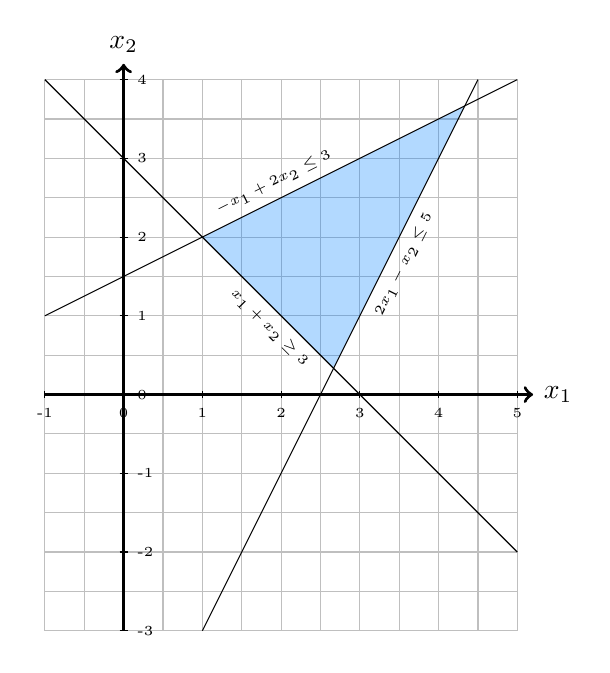
\begin{tikzpicture}
\draw[gray!50, thin, step=0.5] (-1,-3) grid (5,4);
\draw[very thick,->] (-1,0) -- (5.2,0) node[right] {$x_1$};
\draw[very thick,->] (0,-3) -- (0,4.2) node[above] {$x_2$};
%
\foreach \x in {-1,...,5} \draw (\x,0.05) -- (\x,-0.05) node[below] {\tiny\x};
\foreach \y in {-3,...,4} \draw (-0.05,\y) -- (0.05,\y) node[right] {\tiny\y};
%
\fill[blue!50!cyan,opacity=0.3] (8/3,1/3) -- (1,2) -- (13/3,11/3) -- cycle;
%
\draw (-1,4) -- node[below,sloped] {\tiny$x_1+x_2\geq3$} (5,-2);
\draw (1,-3) -- (3,1) -- node[below left,sloped] {\tiny$2x_1-x_2\leq5$} (4.5,4);
\draw (-1,1) -- node[above,sloped] {\tiny$-x_1+2x_2\leq3$} (5,4);
%
\end{tikzpicture}
\par\smallskip
{\footnotesize\raggedright Sumber konstruksi TikZ:
\href{https://tex.stackexchange.com/questions/75933/how-to-draw-the-region-of-inequality}{tex.stackexchange.com/q/75933}.\par}
\caption{Daerah layak program linier generik dengan kendala $x_1+x_2\geq 3$, $2x_1-x_2\leq 5$, dan $-x_1+2x_2\leq 3$. Segitiga berarsir memperlihatkan cara tiga pertidaksamaan linier dapat membentuk daerah poligonal terbatas.}
\label{fig:GenericThreeConstraintRegion}
\end{figure}
%
% Grafik pinjaman dihapus (diganti dengan TikZ hasil reka ulang di atas) -- 13 Mei 2026
% Sebelumnya: \begin{center}\altincludegraphics[width=0.8\linewidth]{images/lemon}{...} \end{center}
% Sumber: external-sources/lineqlpbook/images/lemon.{pdf,svg,fig} (Cheung, CC BY-SA 4.0).
% Gambar lemon.pdf menampilkan program linier Pedagang Limun yang sama dengan
% hasil reka ulang pada gambar TikZ di atas (Gambar~\ref{fig:LemonadeVendorFeasibleRegion}).

Pada Gambar~\ref{fig:LemonadeVendorFeasibleRegion}, kurva aras \(z = 3x+2y\)
digambar untuk beberapa nilai \(z\). Dari gambar, kita dapat melihat bahwa jika \(z\) lebih besar daripada 6.8,
garis yang didefinisikan oleh \(3x+2y = z\) tidak akan berpotongan dengan
daerah layak. Jadi, laba tidak dapat melebihi 6.8 dolar.

Karena garis \(3x+2y = 6.8\) berpotongan dengan daerah layak, \(6.8\)
merupakan nilai maksimum fungsi objektif. Perhatikan bahwa hanya ada satu
titik di daerah layak yang berpotongan dengan garis \(3x+2y=6.8\),
yaitu $(x,y) = (1.2,1.6)$.
Dengan kata lain, untuk memaksimumkan laba, kita perlu membuat 1.2 unit
limun dan 1.6 unit sari lemon.
\end{solution}

Setiap contoh di atas memiliki satu solusi optimal. Namun, terdapat empat hasil yang secara kualitatif berbeda untuk setiap program linier:
\begin{enumerate}[nosep]
\item Solusi optimal tunggal (seperti yang telah kita lihat).
\item Tak terhingga banyak solusi optimal (kurva aras optimal sejajar dengan salah satu sisi daerah layak).
\item Masalah tak berbatas: nilai objektif dapat dibuat sebesar mungkin (maksimisasi) atau sekecil mungkin (minimisasi).
\item Masalah tak layak: tidak ada titik yang memenuhi semua kendala secara bersamaan.
\end{enumerate}

Hasil ketiga hanya dapat terjadi jika daerah layak tak berbatas. Di bawah ini kita akan menggambarkan setiap hasil tersebut dan, pada bab berikutnya, membuktikan bahwa hanya inilah kemungkinan yang ada.

\section{Tak Terhingga Banyak Solusi Optimal}\label{sec:infinitely-many-optima}

Sebuah program linier mungkin memiliki lebih dari satu solusi optimal. Jika ini terjadi, sebenarnya terdapat tak terhingga banyak solusi optimal. Kita menggambarkannya dengan memodifikasi contoh Bengkel Mebel.

\begin{example}{Bengkel Mebel: Objektif Alternatif}\label{exa:FurnitureWorkshopAltOpt}
Misalkan bengkel dalam Contoh~\ref{ex:FurnitureWorkshop} merevisi harganya sehingga setiap kursi menghasilkan \$2 dan setiap meja menghasilkan \$1, serta batas permintaan kursi dinaikkan dari 32 menjadi 35. Fungsi objektif yang baru adalah $z(x_1,x_2) = 2x_1 + x_2$, dan kendalanya menjadi:
\begin{equation}
\begin{aligned}
\max\;\;& z(x_1,x_2) = 2x_1 + x_2\\
\text{dengan syarat}\;\;&  2x_1 + x_2 \leq 80\\
& x_1 + 3x_2 \leq 90\\
& x_1 \leq 35\\
& x_1, x_2 \geq 0
\end{aligned}
\label{eqn:FurnitureWorkshopAltOpt}
\end{equation}
\end{example}

\begin{solution}
Gradien objektif yang baru adalah $\nabla z = (2,1)$, yang tegak lurus terhadap garis kendala $2x_1 + x_2 = 80$; kurva-kurva aras objektif justru sejajar dengan garis kendala tersebut. Ketika kita menyapukan kurva aras ke arah gradien, kurva aras terakhir yang menyentuh daerah layak berimpit dengan seluruh sisi dari $(30,20)$ hingga $(35,10)$. Di sepanjang sisi ini, $2x_1+x_2 = 80$ untuk setiap titik, sehingga $z = 80$ di semua titiknya.

\begin{figure}[H]
\centering
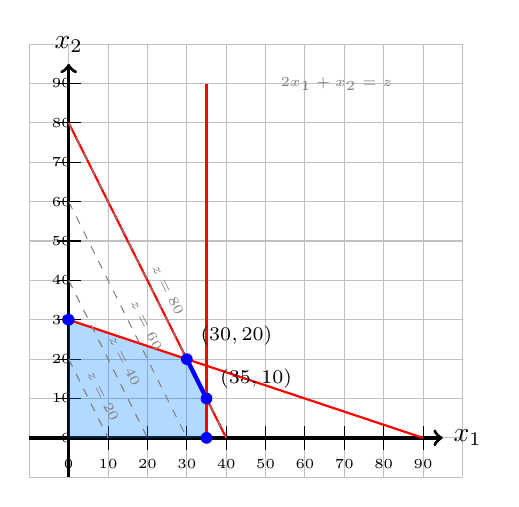
\begin{tikzpicture}[scale=0.05]
    % Kisi dan sumbu
    \draw[gray!50, thin, step=10] (-10,-10) grid (100,100);
    \draw[very thick,->] (-10,0) -- (95,0) node[right] {$x_1$};
    \draw[very thick,->] (0,-10) -- (0,95) node[above] {$x_2$};

    \foreach \x in {0,10,...,90} \draw (\x,3) -- (\x,-3) node[below] {\tiny\x};
    \foreach \y in {0,10,...,90} \draw (-3,\y) -- (3,\y) node[left] {\tiny\y};

    % Daerah layak
    \fill[blue!50!cyan,opacity=0.3]
        (0,0) -- (0,30) -- (30,20) -- (35,10) -- (35,0) -- cycle;

    % Garis kendala
    \draw[red,thick] (0,80) -- (40,0);
    \draw[red,thick] (0,30) -- (90,0);
    \draw[red,thick] (35,90) -- (35,0);

    % Kurva aras (2x1 + x2 = z), kemiringan = -2
    \draw[dashed,gray] (0,20) -- node[pos=0.55,above,sloped] {\tiny $z = 20$} (10,0);
    \draw[dashed,gray] (0,40) -- node[pos=0.55,above,sloped] {\tiny $z = 40$} (20,0);
    \draw[dashed,gray] (0,60) -- node[pos=0.55,above,sloped] {\tiny $z = 60$} (30,0);
    \draw[dashed,gray] (0,80) -- node[pos=0.55,above,sloped] {\tiny $z = 80$} (40,0);

    % Sorot sisi optimal
    \draw[blue,ultra thick] (30,20) -- (35,10);

    % Titik ekstrem
    \node[blue] at (0,30) [circle,fill,inner sep=1.5pt]{};
    \node[blue] at (30,20) [circle,fill,inner sep=1.5pt]{};
    \node[blue] at (35,10) [circle,fill,inner sep=1.5pt]{};
    \node[blue] at (35,0) [circle,fill,inner sep=1.5pt]{};

    \node[black,anchor=south west] at (31,21) {\scriptsize $(30,20)$};
    \node[black,anchor=south west] at (36,10) {\scriptsize $(35,10)$};

    \node[gray] at (68,90) {\tiny $2x_1 + x_2 = z$};
\end{tikzpicture}
\caption{Solusi optimal alternatif: kurva aras $z = 80$ (ruas biru tebal) terletak di sepanjang satu sisi penuh daerah layak. Setiap titik pada sisi ini merupakan solusi optimal.}
\label{fig:FurnitureWorkshopAltOptSoln}
\end{figure}

Misalkan $P$ menyatakan daerah layak. Untuk setiap $x_1^* \in [30,35]$ dengan $x_2^* = 80 - 2x_1^*$, titik $(x_1^*,x_2^*)$ terletak pada sisi dari $(30,20)$ hingga $(35,10)$, dan $z(x_1^*,x_2^*) = 80 \geq z(x_1,x_2)$ untuk semua $(x_1,x_2)\in P$. Karena terdapat tak terhingga banyak titik seperti ini, masalah tersebut memiliki tak terhingga banyak solusi optimal.
\label{ex:FurnitureWorkshopAltOptSoln}
\end{solution}

Berdasarkan contoh ini, kita memperluas algoritma grafis agar dapat menangani beberapa solusi optimal:
\begin{stepbox}{algenter}{\ding{193}\ Metode Grafis 2: Memungkinkan Beberapa Optimum}
\emph{Semua langkah dalam Metode 1, ditambah pemeriksaan nilai yang sama.}
\begin{enumerate}[nosep]
\item Gambar daerah layak dengan memplot batas setiap kendala.
\item Gambar kurva aras fungsi objektif untuk beberapa nilai $z$.
\item Sapukan kurva aras ke arah gradien untuk mencari nilai optimal $z$ yang masih berpotongan dengan daerah layak. Solusi optimal akan terjadi pada sebuah titik ekstrem.
\item Jika kurva aras optimal sejajar dengan sisi daerah layak yang bertemu di titik ekstrem optimal, maka setiap titik pada sisi tersebut juga optimal. Masalah ini memiliki tak terhingga banyak solusi optimal.
\end{enumerate}
\end{stepbox}

\begin{learningcheckpoint}[label={lc:how-many-optima}]
Perhatikan representasi grafis di bawah ini. Berapa banyak solusi optimal yang ada jika kita melakukan maksimisasi? Bagaimana jika kita melakukan minimisasi?
\begin{center}
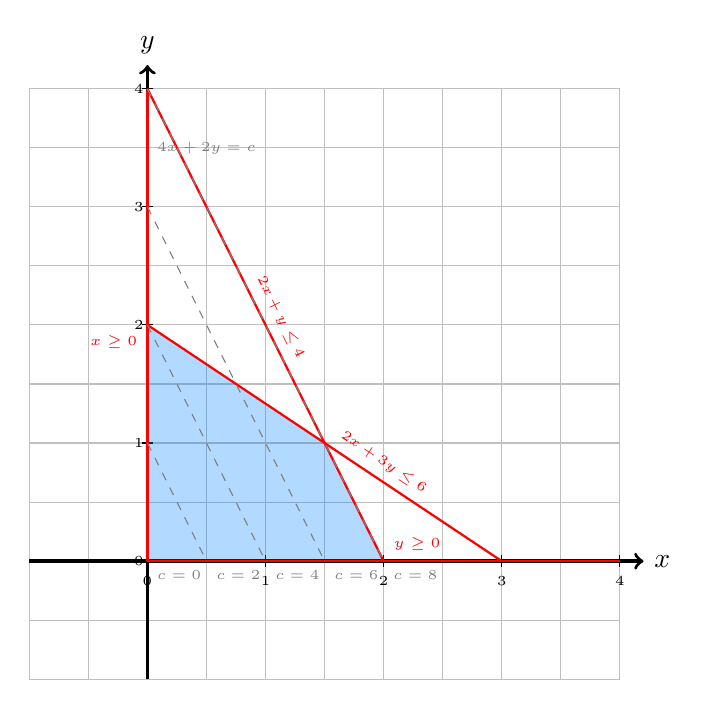
\begin{tikzpicture}[scale = 1.5]
    % Kisi dan sumbu
    \draw[gray!50, thin, step=0.5] (-1,-1) grid (4,4);
    \draw[very thick,->] (-1,0) -- (4.2,0) node[right] {$x$};
    \draw[very thick,->] (0,-1) -- (0,4.2) node[above] {$y$};

    % Label sumbu
    \foreach \x in {0,...,4} \draw (\x,0.05) -- (\x,-0.05) node[below] {\tiny\x};
    \foreach \y in {0,...,4} \draw (-0.05,\y) -- (0.05,\y) node[left] {\tiny\y};

    % Daerah layak yang diarsir
    \fill[blue!50!cyan,opacity=0.3] (0,0) -- (0,2) -- (1.5,1) -- (2,0) -- cycle;

    % Garis kendala
    \draw[red,thick] (0,2) -- node[above right,sloped] {\tiny$2x + 3y \leq 6$} (3,0);
    \draw[red,thick] (0,4) -- node[above,sloped] {\tiny$2x + y \leq 4$} (2,0);
    \draw[red,thick] (0,0) -- node[below left] {\tiny$x \geq 0$} (0,4);
    \draw[red,thick] (0,0) -- node[above right] {\tiny$y \geq 0$} (4,0);

        % Kontur fungsi objektif
            \draw[dashed,gray] (0,4) -- (2,0) node[below right] {\tiny$c=8$};
    \draw[dashed,gray] (0,3) -- (1.5,0) node[below right] {\tiny$c=6$};
    \draw[dashed,gray] (0,2) -- (1,0) node[below right] {\tiny$c=4$};
    \draw[dashed,gray] (0,1) -- (0.5,0) node[below right] {\tiny$c=2$};
    \draw[dashed,gray] (0,0) -- (0,0) node[below right] {\tiny$c=0$};

    % Label kontur
    \node[gray] at (0.5,3.5) {\tiny$4x + 2y = c$};

\end{tikzpicture}
\end{center}
\end{learningcheckpoint}

\section{Masalah Tanpa Solusi}\label{sec:no-solution}

Jika kendala-kendala program linier saling bertentangan, tidak ada titik yang dapat memenuhi semuanya. Daerah layak kosong dan kita menyebut masalah tersebut \emph{tak layak}.

\begin{example}{Masalah Tak Layak}\label{exa:LPInfeasible}
 Perhatikan masalah program linier berikut:
\begin{equation}
\begin{aligned}
\max\;\;& z(x_1,x_2) = 4x_1 + 3x_2\\
\text{dengan syarat}\;\;& x_1 + x_2 \leq 8\\
& 2x_1 + x_2 \leq 12\\
& x_1 \geq 7\\
& x_2 \geq 5
\end{aligned}
\label{eqn:LPInfeasible}
\end{equation}
\end{example}
\begin{solution}
Kendala-kendala tersebut diplot pada Gambar~\ref{fig:LPInfeasible}. Dua kendala pertama membatasi $x_1+x_2\leq 8$, tetapi batas bawah $x_1\geq 7$ dan $x_2\geq 5$ secara bersama-sama mengharuskan $x_1+x_2\geq 12$. Syarat-syarat ini bertentangan, sehingga tidak ada titik yang memenuhi semua kendala secara bersamaan.

\begin{figure}[H]
\centering
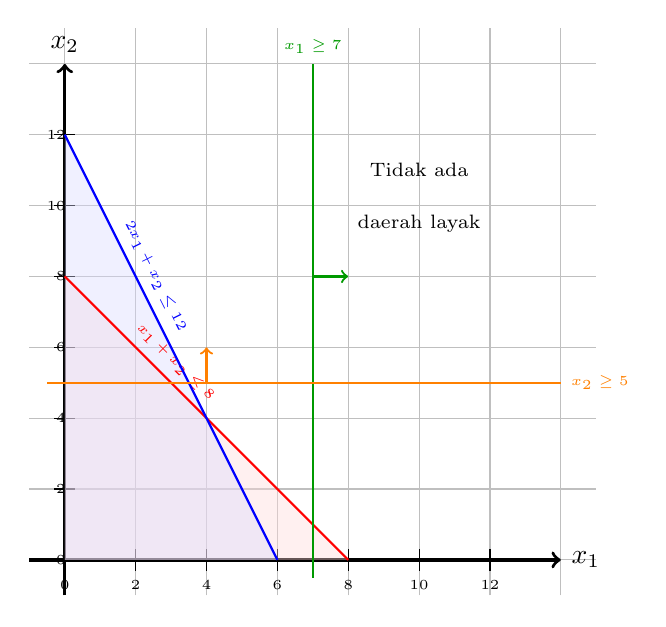
\begin{tikzpicture}[scale=0.45]
    % Kisi dan sumbu
    \draw[gray!50, thin, step=2] (-1,-1) grid (15,15);
    \draw[very thick,->] (-1,0) -- (14,0) node[right] {$x_1$};
    \draw[very thick,->] (0,-1) -- (0,14) node[above] {$x_2$};

    \foreach \x in {0,2,...,12} \draw (\x,0.3) -- (\x,-0.3) node[below] {\tiny\x};
    \foreach \y in {0,2,...,12} \draw (-0.3,\y) -- (0.3,\y) node[left] {\tiny\y};

    % Daerah kendala
    \fill[red!15,opacity=0.4] (0,8) -- (8,0) -- (0,0) -- cycle;
    \fill[blue!15,opacity=0.4] (0,12) -- (6,0) -- (0,0) -- cycle;

    % Garis kendala
    \draw[red,thick] (0,8) -- node[above left, sloped] {\tiny $x_1 + x_2 \leq 8$} (8,0);
    \draw[blue,thick] (0,12) -- node[above left, sloped] {\tiny $2x_1 + x_2 \leq 12$} (6,0);
    \draw[green!60!black,thick] (7,-0.5) -- (7,14) node[above] {\tiny $x_1 \geq 7$};
    \draw[orange,thick] (-0.5,5) -- (14,5) node[right] {\tiny $x_2 \geq 5$};

    % Panah yang menunjukkan arah yang diwajibkan
    \draw[->,green!60!black,thick] (7,8) -- (8,8);
    \draw[->,orange,thick] (4,5) -- (4,6);

    % Label ketaklayakan
    \node[black] at (10,11) {\scriptsize Tidak ada};
    \node[black] at (10,9.5) {\scriptsize daerah layak};
\end{tikzpicture}
\caption{Program linier yang tak layak. Kendala batas atas memaksakan $x_1+x_2\leq 8$, tetapi batas bawah mengharuskan $x_1\geq 7$ dan $x_2\geq 5$, sehingga $x_1+x_2\geq 12$. Tidak ada titik yang dapat memenuhi kedua syarat, dan daerah layak kosong.}
\label{fig:LPInfeasible}
\end{figure}

Karena daerah layak kosong, masalah tersebut tidak mempunyai solusi.
\label{ex:LPNoSoln}
\end{solution}
Sebelum menyatakan algoritma grafis yang lengkap, kita juga membahas kasus daerah layak tak berbatas.

\section{Masalah dengan Daerah Layak Tak Berbatas}\label{sec:unbounded-regions}

Perhatikan masalah berikut:

\begin{align*}
\min \quad && z = 5x_1 + 7x_2  \\
\text{dengan syarat} \quad && x_1 + 3x_2 &\geq 6 \\
&& 5x_1 + 2x_2 &\geq 10 \\
&& x_2 &\leq 4 \\
&& x_1, x_2 &\geq 0
\end{align*}

\begin{center}
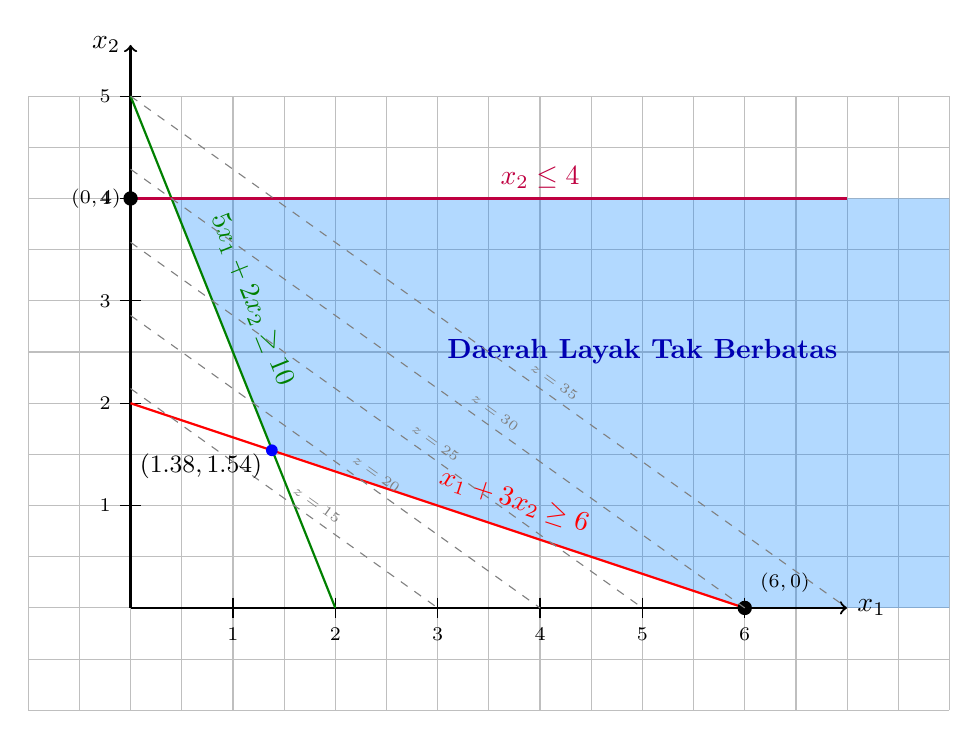
\begin{tikzpicture}[scale = 1.3]
    \draw[gray!50, thin, step=0.5] (-1,-1) grid (8,5);

    % Sorot daerah layak
    \fill[blue!50!cyan,opacity=0.3]
        (0.4,4) -- (1.39,1.55)  -- (6,0) -- (8,0) -- (8,4) -- cycle;

    % Definisikan sumbu
    \draw[thick,->] (0,0) -- (7,0) node[right] {$x_1$};
    \draw[thick,->] (0,0) -- (0,5.5) node[anchor=east] {$x_2$};

    % Tambahkan tanda skala pada sumbu x_1
    \foreach \x in {1,2,3,4,5,6} {
        \draw (\x,0.1) -- (\x,-0.1) node[anchor=north] {\scriptsize $\x$};
    }

    % Tambahkan tanda skala pada sumbu x_2
    \foreach \y in {1,2,3,4,5} {
        \draw (0.1,\y) -- (-0.1,\y) node[anchor=east] {\scriptsize $\y$};
    }

    % Definisikan kendala
    % Garis 1: X + 3Y = 6
    \draw[red,thick] (0,2) -- (6,0);
    \node[red, rotate=-18, anchor=north west] at (3,1.5) {$x_1 + 3x_2 \geq 6$};

    % Garis 2: 5X + 2Y = 10
    \draw[green!50!black,thick] (0,5) -- (2,0);
    \node[green!50!black, rotate=-68, anchor=north west] at (1,4) {$5x_1 + 2x_2 \geq 10$};

    % Garis 3: Y = 4
    \draw[purple,thick] (0,4) -- (7,4);
    \node[purple, rotate=0, anchor=south] at (4,4) {$x_2 \leq 4$};

    % Label daerah layak
    \node[blue!70!black, font=\bfseries] at (5,2.5) {Daerah Layak Tak Berbatas};

    % Tandai titik perpotongan
\fill[black] (0,4) circle (2pt) node[anchor=east] {\scriptsize $(0,4)$};
\fill[black] (6,0) circle (2pt) node[anchor=south west,xshift=2pt,yshift=2pt] {\scriptsize $(6,0)$};

% Kontur fungsi objektif
\foreach \c in {15,20,25,30,35} {
    \draw[dashed,gray] (0,\c/7) -- node[pos=0.58,above,sloped] {\tiny$z = \c$} (\c/5,0);
    }
\node[blue,circle,fill,inner sep=1.5pt,label={[black,anchor=north east]\small$(1.38,1.54)$}] at (1.38,1.54) {};

\end{tikzpicture}
\end{center}

%% Gambar asli dihapus (berkas tidak tersedia)

Seperti terlihat, daerah layaknya \emph{tak berbatas}. Secara khusus, dari titik mana pun di daerah layak, kita selalu dapat menemukan titik layak lain dengan meningkatkan koordinat $x_1$ (yakni bergerak ke kanan pada gambar). Namun, ini tidak selalu berarti bahwa masalah optimisasinya tak berbatas.

Kenyataannya, solusi optimal berada pada $\mathbf{x}^* = (1.38, 1.54)$, titik ekstrem di sudut kiri bawah,
dengan nilai objektif optimal
$$
z^* = 5 \cdot 1.38 + 7\cdot 1.54 = 17.7.
$$

Namun, pertimbangkan masalah lain, yaitu ketika kita mencoba memaksimumkan objektif
\begin{align*}
{\color{red} \max }\quad && z = 5x_1 + 7x_2  \\
\text{dengan syarat} \quad && x_1 + 3x_2 &\geq 6 \\
&& 5x_1 + 2x_2 &\geq 10 \\
&& x_2 &\leq 4 \\
&& x_1, x_2 &\geq 0
\end{align*}

\begin{solution}
Masalah optimisasi ini tak berbatas! Sebagai contoh, perhatikan bahwa titik $(x_1,x_2) = (n,0)$ layak untuk setiap bilangan bulat $n\geq 6$. Maka fungsi objektif $z = 5n + 0$ mengikuti barisan $30, 35, 40, \dots$, yang divergen menuju tak hingga.
\end{solution}

Sekarang kita menggambarkan dua skenario lain dengan daerah layak tak berbatas. Pada skenario pertama, masalahnya tak berbatas; pada skenario kedua, optimum hingga tetap ada walaupun daerahnya tak berbatas.

\begin{example}{Masalah Tak Berbatas}\label{ex:LPUnboundFeasibleRegion1} Perhatikan masalah program linier berikut:
\begin{equation}
\begin{aligned}
\max\;\;& z(x_1,x_2) = x_1 + 3x_2\\
\text{dengan syarat}\;\;& x_1 - x_2 \leq 3\\
& x_1 + 2x_2 \geq 4\\
&x_1,x_2 \geq 0
\end{aligned}
\label{eqn:LPUnboundFeasibleRegion1}
\end{equation}
\end{example}
\begin{solution}
Daerah layak dan kurva aras ditunjukkan pada Gambar~\ref{fig:LPUnboundFeasibleRegion1}.

\begin{figure}[H]
\centering
\begin{tikzpicture}[scale = 0.9]
    \draw[gray!50, thin, step=1] (-1,-1) grid (9,8);
    \draw[very thick,->] (-1,0) -- (9,0) node[right] {$x_1$};
    \draw[very thick,->] (0,-1) -- (0,8) node[above] {$x_2$};

    \foreach \x in {0,...,8} \draw (\x,0.05) -- (\x,-0.05) node[below] {\tiny\x};
    \foreach \y in {0,...,7} \draw (-0.05,\y) -- (0.05,\y) node[left] {\tiny\y};

    % Daerah layak (tak berbatas ke atas-kanan)
    % Titik ekstrem: (0,2), (10/3, 1/3), lalu memanjang sepanjang kedua garis batas
    \fill[blue!50!cyan,opacity=0.3] (0,2) -- (10/3,1/3) -- (9,6) -- (9,8) -- (0,8) -- cycle;

    % Garis kendala, dipotong pada bingkai plot agar tidak menjorok ke keterangan.
    \begin{scope}
    \clip (-1,-1) rectangle (9,8);
    \draw[red,thick] (0,-3) -- node[below right,sloped,pos=0.7] {\tiny$x_1 - x_2 \leq 3$} (8,5);
    \draw[red,thick] (4,0) -- node[below left,sloped,pos=0.3] {\tiny$x_1 + 2x_2 \geq 4$} (0,2);
    \draw[red,thick] (0,0) -- node[pos=0.66,right] {\tiny$x_1 \geq 0$} (0,8);
    \end{scope}

    % Kurva aras (x1 + 3x2 = z)
    \draw[dashed,gray] (3,0) -- node[pos=0.25,above,sloped] {\tiny$z=3$} (0,1);
    \draw[dashed,gray] (6,0) -- node[pos=0.25,above,sloped] {\tiny$z=6$} (0,2);
    \draw[dashed,gray] (9,0) -- node[pos=0.25,above,sloped] {\tiny$z=9$} (0,3);
    \draw[dashed,gray] (9,1) -- node[pos=0.25,above,sloped] {\tiny$z=12$} (0,4);
    \draw[dashed,gray] (9,2) -- node[pos=0.25,above,sloped] {\tiny$z=15$} (0,5);

    \node[gray] at (6,7) {\tiny$x_1 + 3x_2 = z$};

    % Titik ekstrem
    \node[blue] at (0,2) [circle,fill,inner sep=1.5pt]{};
    \node[blue] at (10/3,1/3) [circle,fill,inner sep=1.5pt]{};
    \node[black,anchor=south east] at (0,2) {\scriptsize$(0,2)$};
    \node[black,anchor=south east] at (3.2,0.7) {\scriptsize$(\tfrac{10}{3},\tfrac{1}{3})$};
\end{tikzpicture}
\caption{Program linier tak berbatas. Daerah layak memanjang tak hingga ke atas dan ke kanan. Kurva aras $z = x_1 + 3x_2$ tetap berpotongan dengan daerah layak untuk nilai $z$ sebesar apa pun, sehingga masalah tersebut tak berbatas.}
\label{fig:LPUnboundFeasibleRegion1}
\end{figure}

Daerah layak memanjang tak hingga ke atas dan ke kanan. Untuk setiap nilai sasaran $z_0$, kita dapat menemukan titik layak yang mencapai $z \geq z_0$. Sebagai contoh, ambil $(x_1,x_2) = (0,t)$ untuk $t\geq 2$: maka $0-t = -t \leq 3$ dan $0+2t = 2t\geq 4$, sehingga titik tersebut layak, dan $z = 3t$, yang meningkat tanpa batas. Jadi, nilai optimalnya adalah $+\infty$ dan masalah tersebut tak berbatas.
\end{solution}

Daerah layak yang tak berbatas tidak selalu menghasilkan objektif tak berbatas. Hal yang menentukan ialah apakah gradien objektif menunjuk ke arah tak berbatas atau menjauhinya.

\begin{example}{Optimum Hingga dengan Daerah Layak Tak Berbatas}\label{exa:LPUnboundFiniteSoln}
Perhatikan daerah layak yang sama seperti dalam Contoh~\ref{ex:LPUnboundFeasibleRegion1}, tetapi dengan objektif baru:
\begin{equation}
\begin{aligned}
\min\;\;& z(x_1,x_2) = 3x_1 + x_2\\
\text{dengan syarat}\;\;& x_1 - x_2 \leq 3\\
& x_1 + 2x_2 \geq 4\\
&x_1,x_2 \geq 0
\end{aligned}
\label{eqn:LPUnboundFiniteSoln}
\end{equation}
\end{example}
\begin{solution}
Daerah layaknya merupakan daerah tak berbatas yang sama seperti sebelumnya. Namun, sekarang kita melakukan \emph{minimisasi}, dan gradien $(3,1)$ menunjuk ke kanan dan sedikit ke atas, tepat menuju bagian daerah layak yang tak berbatas. Bergerak berlawanan dengan gradien (menuju $z$ yang lebih kecil) membawa kita ke sudut kiri bawah daerah layak.

\begin{figure}[H]
\centering
\begin{tikzpicture}[scale = 0.9]
    \draw[gray!50, thin, step=1] (-1,-1) grid (9,8);
    \draw[very thick,->] (-1,0) -- (9,0) node[right] {$x_1$};
    \draw[very thick,->] (0,-1) -- (0,8) node[above] {$x_2$};

    \foreach \x in {0,...,8} \draw (\x,0.05) -- (\x,-0.05) node[below] {\tiny\x};
    \foreach \y in {0,...,7} \draw (-0.05,\y) -- (0.05,\y) node[left] {\tiny\y};

    % Daerah layak
    \fill[blue!50!cyan,opacity=0.3] (0,2) -- (10/3,1/3) -- (9,6) -- (9,8) -- (0,8) -- cycle;

    % Garis kendala, dipotong pada bingkai plot agar tidak menjorok ke keterangan.
    \begin{scope}
    \clip (-1,-1) rectangle (9,8);
    \draw[red,thick] (0,-3) -- (8,5);
    \draw[red,thick] (4,0) -- (0,2);
    \draw[red,thick] (0,0) -- (0,8);
    \end{scope}

    % Kurva aras (3x1 + x2 = z)
    \draw[dashed,gray] (0,2) -- node[pos=0.55,above,sloped] {\tiny$z=2$} (2/3,0);
    \draw[dashed,gray] (0,4) -- node[pos=0.55,above,sloped] {\tiny$z=4$} (4/3,0);
    \draw[dashed,gray] (0,6) -- node[pos=0.55,above,sloped] {\tiny$z=6$} (2,0);
    \draw[dashed,gray] (0,8) -- node[pos=0.55,above,sloped] {\tiny$z=8$} (8/3,0);

    \node[gray] at (5,7) {\tiny$3x_1 + x_2 = z$};

    % Titik ekstrem optimal
    \node[blue] at (0,2) [circle,fill,inner sep=2pt]{};
    \node[black,anchor=south east] at (-0.2,2) {\scriptsize$(0,2)$};
    \node[blue] at (10/3,1/3) [circle,fill,inner sep=1.5pt]{};
    \node[black,anchor=south east] at (3.2,0.7) {\scriptsize$(\tfrac{10}{3},\tfrac{1}{3})$};
\end{tikzpicture}
\caption{Program linier dengan daerah layak tak berbatas, tetapi memiliki solusi optimal hingga. Minimum $z = 3x_1+x_2$ terjadi pada titik ekstrem $(0,2)$ dengan $z^* = 2$, karena gradien menunjuk menjauhi ujung daerah layak yang terbatas.}
\label{fig:LPUnboundFeasibleRegion2}
\end{figure}

Evaluasi objektif pada titik-titik ekstrem memberikan $z(0,2) = 2$ dan $z(\tfrac{10}{3},\tfrac{1}{3}) = 10 + \tfrac{1}{3} = \tfrac{31}{3} \approx 10.3$. Karena kita melakukan minimisasi, optimumnya adalah $z^* = 2$ pada $(x_1^*,x_2^*) = (0,2)$. Sekali lagi, solusi optimal terjadi pada sebuah titik ekstrem daerah layak, walaupun daerah tersebut tak berbatas.
\label{ex:LPUnboundFeasibleRegion2}
\end{solution}

Sekarang kita dapat menyatakan algoritma lengkap untuk menyelesaikan setiap program linier dua variabel secara grafis.

\begin{stepbox}{algopt}{\ding{51}\ Metode Grafis Lengkap untuk Program Linier Dua Variabel}
\emph{Menangani setiap kasus: tak layak, tak berbatas, optimum tunggal, dan beberapa optimum.}
\begin{enumerate}
    \item Gambar daerah layak dengan memplot batas-batas kendala dan mengarsir perpotongannya.
    \item Jika daerah layak kosong, masalah tersebut \textbf{tak layak}; berhenti.
    \item Gambar kurva aras fungsi objektif dan tentukan arah gradien.
    \item \textbf{Daerah layak terbatas:}
    \begin{enumerate}
        \item Sapukan kurva aras ke arah gradien (untuk maksimisasi) atau berlawanan dengannya (untuk minimisasi) hingga ditemukan kurva aras terakhir yang menyentuh daerah layak. Solusi optimal berada pada sebuah titik ekstrem.
        \item Jika kurva aras optimal ini sejajar dengan sebuah sisi daerah layak, setiap titik pada sisi tersebut optimal (tak terhingga banyak solusi).
    \end{enumerate}
    \item \textbf{Daerah layak tak berbatas:}
    \begin{enumerate}
        \item Jika kurva aras dapat disapukan tanpa batas sambil tetap berpotongan dengan daerah layak, masalah tersebut \textbf{tak berbatas}.
        \item Jika tidak, optimum hingga berada pada sebuah titik ekstrem; lanjutkan seperti pada kasus terbatas.
    \end{enumerate}
\end{enumerate}
\end{stepbox}

\newpage

\section{Latihan}\label{exercises}

\exgroup{Pemanasan}

\begin{ex}{Analisis Daerah Layak}{}
\stars{1}Perhatikan sistem kendala berikut:
\[
x + y \geq 5
\]
\[
x \geq 0, \quad y \geq 0
\]
Manakah pernyataan berikut yang benar mengenai daerah layaknya?
\begin{enumerate}
    \item Daerah layak merupakan poligon terbatas.
    \item Daerah layak merupakan daerah tak berbatas.
    \item Daerah layak terdiri atas satu titik.
    \item Masalah tersebut tak layak.
\end{enumerate}
\exrefs{\S\ref{sec:nonempty-bounded}, \S\ref{sec:unbounded-regions}}
\end{ex}

\begin{ex}{Menggambar Daerah Layak}{}\label{ex:feasible-region}
\stars{1}Gambarkan semua \(\begin{bmatrix} x \\ y \end{bmatrix}\) yang memenuhi
\[
x - 2y \leq 2
\]
pada bidang \((x,y)\).
\exrefs{\S\ref{sec:nonempty-bounded}}
\end{ex}

\begin{ex}{Latihan Metode Grafis 1}{}\label{ex:graphical-method-one}
\stars{1}Terapkan langkah-langkah pada kotak ``Metode Grafis 1: Daerah Terbatas, Optimum Tunggal'' terhadap program linier
\begin{align*}
\max \quad & 3x + 2y\\
\text{dengan syarat} \quad & x + y \leq 4\\
& x \leq 3\\
& x, y \geq 0.
\end{align*}
Gambarkan daerah layak, daftarkan keempat titik ekstremnya, lalu sapukan kurva aras $z = 3x + 2y$ ke arah gradien untuk menemukan solusi optimal dan nilai optimal.
\exrefs{\S\ref{sec:graphical-approach}, Contoh~\ref{ex:FurnitureWorkshop}}
\end{ex}

\begin{ex}{Metode Grafis untuk Pedagang Limun}{}
\stars{1}Selesaikan masalah Pedagang Limun dari Contoh~\ref{exa:lemonadevendor} dengan metode grafis.
\exrefs{\S\ref{sec:graphical-approach}, Contoh~\ref{exa:lemonadevendor}}
\end{ex}

\Needspace{6\baselineskip}
\exgroup{Masalah inti}

\begin{ex}{Metode Grafis}{}
\stars{2}Gunakan metode grafis untuk menentukan dua solusi optimal bagi program linier berikut:
\begin{align*}
\min  \quad& 3x_1 + 5x_2\\
 & 3x_1 + 2x_2 \ge 36\\
 & 6x_1 + 10x_2 \geq 90\\
 & x_1, x_2 \geq 0
\end{align*}
\exrefs{\S\ref{sec:infinitely-many-optima}, Contoh~\ref{exa:FurnitureWorkshopAltOpt}}
\end{ex}

\begin{ex}{Grafik Daerah Tak Layak}{}\label{ex:infeasible}
\stars{2}Gambarkan daerah layak program linier berikut:
\begin{align*}
\min  \quad & x_1 - x_2\\
 & x_1 + x_2 \leq 6\\
 & x_1 - x_2 \geq 1\\
 & x_2 - x_1 \geq 3\\
 & x_1, x_2 \geq 0
\end{align*}
Tanpa mempertimbangkan fungsi objektif, berapa banyak solusi layak yang ada? Berikan alasan atas jawaban Anda.
\exrefs{\S\ref{sec:no-solution}, Contoh~\ref{exa:LPInfeasible}}
\end{ex}

\begin{ex}{Menentukan Nilai Optimal}{}\label{ex:lp-optimal-value}
\stars{2}Tentukan nilai optimal dari
\[
\begin{array}{rl}
\text{Minimumkan} & x + y \\
\text{Dengan syarat} &  2x + y \geq 4 \\
& x + 3y \geq 1.
\end{array}
\]
\exrefs{\S\ref{sec:graphical-approach}}
\end{ex}

\begin{ex}{Menunjukkan Masalah Tak Berbatas}{}\label{ex:lp-unbounded}
\stars{2}Tunjukkan bahwa masalah
\[
\begin{array}{rl}
\text{Minimumkan} & -x + y \\
\text{Dengan syarat} &  2x - y \geq 0 \\
& x + 3y \geq 3
\end{array}
\]
tak berbatas.
\exrefs{\S\ref{sec:unbounded-regions}, Contoh~\ref{ex:LPUnboundFeasibleRegion1}}
\end{ex}

\begin{ex}{Berhingga atau Tak Berbatas?}{}\label{exer:BoundedSolutionQuestion}
\stars{2}Perhatikan daerah layak dari Contoh~\ref{ex:LPUnboundFeasibleRegion1} (dengan $x_1-x_2\leq 3$ dan $x_1+2x_2\geq 4$). Apakah masalah $\max\; z = -2x_1 + x_2$ dengan kendala-kendala tersebut mempunyai solusi hingga? Berikan alasan dengan menggunakan Metode Grafis Lengkap.
\exrefs{\S\ref{sec:unbounded-regions}, Contoh~\ref{exa:LPUnboundFiniteSoln}}
\end{ex}

\begin{ex}{Masalah Diet}{}\label{ex:lp-diet-problem}
\stars{2}Misalkan Anda berbelanja suplemen makanan untuk memenuhi
kebutuhan asupan harian 0.40 mg nutrien \(M\) dan 0.30 mg
nutrien \(N\). Ada tiga produk populer di pasaran. Biaya dan jumlah
kedua nutrien dalam tiap produk diberikan pada tabel berikut:

\begin{table}[h!]
\centering
\begin{tabular}{lccc}
\toprule
         & Produk 1 & Produk 2 & Produk 3 \\ \midrule
Biaya     & \$27      & \$31      & \$24      \\
Jumlah harian \(M\) & 0.16 mg   & 0.21 mg   & 0.11 mg   \\
Jumlah harian \(N\) & 0.19 mg   & 0.13 mg   & 0.15 mg   \\ \bottomrule
\end{tabular}
\caption{Data untuk masalah.}
\label{tab:your_table_label}
\end{table}

Anda ingin menentukan banyaknya setiap produk yang perlu dibeli agar
kebutuhan asupan harian kedua nutrien terpenuhi dengan biaya minimum.
Rumuskan masalah ini sebagai masalah program linier dengan asumsi bahwa
Anda dapat membeli produk dalam jumlah pecahan.
\exrefs{\S\ref{sec:graphical-approach}, Contoh~\ref{exa:lemonadevendor}}
\end{ex}

\exgroup{Konsep dan keterkaitan}

\begin{ex}{Mengapa Optimum Harus Berada pada Titik Ekstrem?}{}\label{ex:why-vertex}
\stars{2}Misalkan sebuah program linier dalam dua variabel mempunyai daerah layak yang tak kosong dan terbatas.
\begin{enumerate}
\item Teorema~\ref{thm:optimalextremepoint} menjamin bahwa suatu solusi optimal terjadi pada titik ekstrem. Dengan menggunakan gambaran kurva aras, jelaskan alasannya: jika sebuah titik layak terletak tepat di bagian dalam daerah, atau tepat di bagian dalam suatu sisi, mengapa kita selalu dapat menemukan titik ekstrem yang nilai objektifnya sekurang-kurangnya sama baik?
\item Bagian mana dari argumen Anda yang menggunakan asumsi bahwa daerah tersebut terbatas? Berikan contoh daerah layak tak berbatas dan fungsi objektif yang sama sekali tidak memiliki solusi optimal.
\end{enumerate}
\exrefs{\S\ref{sec:nonempty-bounded}, Teorema~\ref{thm:optimalextremepoint}}
\end{ex}

\begin{ex}{Solusi Optimal Tak Terhingga Banyak}{}
\stars{2}Temukan fungsi objektif untuk daerah layak dalam Contoh~\ref{ex:LPUnboundFeasibleRegion1} yang menghasilkan tak terhingga banyak solusi optimal. Jelaskan himpunan optimumnya.
\exrefs{\S\ref{sec:infinitely-many-optima}}
\end{ex}

\begin{ex}{Tak Terhingga Banyak Solusi Optimal}{}
\stars{2}Ubah fungsi objektif dalam Contoh~\ref{exa:lemonadevendor} sehingga program linier yang dihasilkan memiliki tak terhingga banyak solusi optimal. Jelaskan himpunan lengkap solusi optimalnya.
\exrefs{\S\ref{sec:infinitely-many-optima}, Contoh~\ref{exa:lemonadevendor}}
\end{ex}

\begin{ex}{Optimum Terbatas pada Daerah Tak Berbatas}{}
\stars{2}Perhatikan kendala $-x_1+x_2\leq 5$, $x_1+x_2\geq 2$, $x_1,x_2\geq 0$. Bentuklah sebuah objektif \textbf{maksimisasi} yang mempunyai optimum hingga meskipun daerah layaknya tak berbatas. Gambarkan daerah layak dan kurva aras untuk memverifikasinya.

\emph{[Petunjuk: Pilih gradien yang menunjuk menjauhi arah tak berbatas.]}
\exrefs{\S\ref{sec:unbounded-regions}, Contoh~\ref{exa:LPUnboundFiniteSoln}}
\end{ex}

\Needspace{6\baselineskip}
\exgroup{Masalah tantangan}

\begin{ex}{Arah Objektif Tak Berbatas}{}
\stars{3}Perhatikan masalah berikut:
\[
\begin{array}{rrcrll}
\text{minimumkan } & -2x_1 & + & x_2 & \\
\text{dengan syarat} & -x_1 & + & x_2 & \leq & 3 \\
& x_1 & - & 2x_2 & \leq & 2 \\
& x_1 & & & \geq & 0 \\
& & & x_2 & \geq & 0. \\
\end{array}
\]

\begin{enumerate}
\item Tunjukkan bahwa untuk setiap \(t \geq 0\),
\[
\begin{bmatrix} x_1 \\ x_2 \end{bmatrix} = \begin{bmatrix} t \\ t \end{bmatrix}
\]
memenuhi semua kendala. Tunjukkan bahwa fungsi objektif tak berbatas pada titik ini ketika $t \to \infty$.

\item Tunjukkan bahwa \[
\begin{bmatrix} x_1 \\ x_2 \end{bmatrix} = \begin{bmatrix} 2t+2 \\ t \end{bmatrix}
\]
 layak untuk setiap \(t \geq 0\). Berapakah nilai fungsi objektif pada titik ini? Tunjukkan lagi bahwa fungsi objektif tak berbatas dengan mengambil $t \to \infty$.
 \end{enumerate}
\exrefs{\S\ref{sec:unbounded-regions}, Contoh~\ref{ex:LPUnboundFeasibleRegion1}}
 \end{ex}

\begin{ex}{Optimisasi Terbatas dan Tak Berbatas}{}
\stars{3}Perhatikan masalah berikut:

\[
\begin{array}{rrcllll}
\text{maksimumkan/minimumkan } & 2x & + & 2y \\
\text{dengan syarat} & -x & + & 2y & \leq & 12 \\
& 2x & + & y & \geq & 4 \\
& x & + & 2y & \geq & 5 \\
& x & & & \geq & 0 \\
& & & y & \geq & 0. \\
\end{array}
\]

\begin{enumerate}

\item Tentukan nilai minimum \(2x + 2y\) dengan menyelesaikan masalah optimisasi terkait secara grafis. Tunjukkan bahwa minimum dicapai pada suatu titik layak yang terbatas.

\item Tunjukkan bahwa nilai maksimum \(2x + 2y\) tak berbatas dengan mencari solusi layak berbentuk
\[
\begin{bmatrix} x \\ y \end{bmatrix} = \begin{bmatrix} 5\\ 0\end{bmatrix} + t \begin{bmatrix} 1\\ 0\end{bmatrix}
\]
untuk setiap \(t \geq 0\). Tunjukkan bahwa ketika \(t \to \infty\), fungsi objektif menjadi tak berbatas.

\item Tunjukkan bahwa
\[
\begin{bmatrix} x \\ y \end{bmatrix} = \begin{bmatrix} 0 \\ 6 \end{bmatrix} + t\begin{bmatrix} 2 \\ 1 \end{bmatrix}
\]
layak untuk setiap \(t \geq 0\). Hitung nilai fungsi objektif pada titik ini dan tunjukkan bahwa nilainya tak berbatas ketika \(t \to \infty\).

\end{enumerate}
\exrefs{\S\ref{sec:unbounded-regions}}
\end{ex}

\begin{ex}{Dari Sisi Optimal ke Optimum Tunggal}{}\label{ex:edge-of-optima}
\stars{3}Buatlah agar beberapa solusi optimal memiliki nilai yang sama, lalu hilangkan kesamaan tersebut.
\begin{enumerate}
\item Bentuklah program linier dalam dua variabel yang himpunan solusi optimalnya berupa satu sisi penuh daerah layak, bukan hanya satu titik ekstrem. Gambarkan daerah layak, tentukan sisi optimalnya, dan gunakan langkah pemeriksaan nilai yang sama dalam Metode Grafis 2 untuk menjelaskan mengapa setiap titik pada sisi tersebut optimal.
\item Sekarang ubah tepat satu koefisien dalam fungsi objektif sehingga program linier yang telah dimodifikasi mempunyai solusi optimal tunggal pada sebuah titik ekstrem dari daerah layak yang sama. Tentukan titik ekstrem optimal yang baru dan jelaskan mengapa kesamaan nilai tersebut hilang.
\end{enumerate}
\exrefs{\S\ref{sec:infinitely-many-optima}, Contoh~\ref{exa:FurnitureWorkshopAltOpt}}
\end{ex}

%Oleh Kevin Cheung
%Buku ini dilisensikan berdasarkan
%\href{http://creativecommons.org/licenses/by-sa/4.0/}{Lisensi Internasional Creative Commons
%Atribusi-BerbagiSerupa 4.0}.
%
%Berkas ini dimodifikasi oleh Robert Hildebrand pada 2020.
%Lisensi CC BY-SA 4.0 tetap berlaku.

% Fragmen lama, seluruhnya dijadikan komentar pada 2026-07-08
%\section{Contoh grafis}\label{graphic}
%
%Untuk memotivasi pokok bahasan program linier (PL), kita mulai dengan
%masalah perencanaan yang dapat diselesaikan secara grafis.
%
%
%
%Metode penyelesaian di atas sulit dianggap ketat karena kita
%mengandalkan gambar untuk menyimpulkan bahwa \(3x + 2y \leq 6.8\) bagi semua
%$(x,y)$ yang memenuhi kendala. Namun, sebenarnya kita dapat menunjukkan hal ini
%secara \emph{aljabar}.
%
%Perhatikan bahwa mengalikan kedua ruas kendala \(x + 3y \leq 6\)
%menghasilkan \(0.2x + 0.6 y \leq 1.2\), dan mengalikan kedua ruas
%kendala \(2x + y \leq 4\) menghasilkan \(2.8x + 1.4 y \leq 5.6\). Jadi, setiap
%\(\begin{bmatrix} x\\y\end{bmatrix}\) yang memenuhi \(x+3y\leq 6\)
%dan \(2x+y \leq 4\) juga harus memenuhi
%\((0.2x+0.6y) + (2.8x+1.4y) \leq 1.2 + 5.6\), yang disederhanakan menjadi
%\(3x + 2y \leq 6.8\), seperti yang diinginkan! (Di sini kita menggunakan fakta bahwa jika
%\(a \leq b\) dan \(c \leq d\), maka \(a+c \leq b+d\).)
%
%Sekarang, kita mungkin bertanya apakah bukti aljabar seperti di atas
%selalu dapat ditemukan untuk masalah serupa. Jika jawabannya ya, bagaimana
%cara menemukan bukti seperti itu? Kita akan melihat jawabannya nanti.
%
%Sebelum mengakhiri bagian ini, perhatikan masalah berikut:
%\[\begin{array}{rrcrll}
%\text{minimumkan } & -2x & + & y & \\
%\text{dengan syarat} & -x & + & y & \leq & 3 \\
%& x & - &  2y & \leq & 2 \\
%& x &  & & \geq & 0 \\
%& & & y & \geq & 0. \\
%\end{array}\]
%
%Perhatikan bahwa untuk setiap \(t \geq 0\),
%\(\begin{bmatrix} x \\ y\end{bmatrix} = \begin{bmatrix} t \\ t\end{bmatrix}\)
%memenuhi semua kendala. Nilai fungsi objektif pada
%\(\begin{bmatrix} x \\ y\end{bmatrix} = \begin{bmatrix} t \\ t\end{bmatrix}\)
%adalah \(-t\). Ketika \(t \rightarrow \infty\), nilai fungsi objektif
%menuju \(-\infty\). Oleh karena itu, fungsi objektif tidak memiliki nilai minimum.
%Masalah tersebut dikatakan tak berbatas. Kelak kita akan mempelajari cara
%mendeteksi ketakberbatasan secara algoritmis.
%
%Sebagai latihan, periksa bahwa ketakberbatasan juga dapat dibuktikan dengan
%menggunakan
%\(\begin{bmatrix} x \\ y\end{bmatrix} = \begin{bmatrix} 2t+2 \\ t\end{bmatrix}\)
%untuk \(t \geq 0\).



\subsubsection*{Solusi Terpilih}
\label{solutions}
\addcontentsline{toc}{subsection}{Solusi}

\begin{solution}(Latihan~\ref{ex:graphical-method-one})
Daerah layak memiliki titik-titik ekstrem $(0,0)$, $(3,0)$, $(3,1)$, dan $(0,4)$. Evaluasi objektif memberikan $z(0,0)=0$, $z(3,0)=9$, $z(3,1)=11$, dan $z(0,4)=8$. Dengan menyapukan kurva aras $z = 3x+2y$ ke arah gradien $(3,2)$, kurva aras terakhir yang menyentuh daerah tersebut melewati $(3,1)$, tempat kendala $x+y\leq 4$ dan $x\leq 3$ sama-sama aktif. Solusi optimalnya adalah $(x^*,y^*) = (3,1)$ dengan nilai optimal $z^* = 11$.
\end{solution}

\begin{solution}(Latihan~\ref{ex:infeasible})
Kenyataannya, kendala 2 dan 3 menunjuk ke arah yang saling menjauh sehingga tidak ada solusi layak.
\end{solution}

\begin{solution}(Latihan \ref{ex:feasible-region})

Titik-titik \((x,y)\) yang memenuhi \(x-2y \leq 2\) tepat merupakan titik-titik
di atas garis yang melalui \((2,0)\) dan \((0,-1)\).
\end{solution}

\begin{solution}(\ref{ex:lp-optimal-value})

Kita ingin menentukan nilai minimum \(z\) sedemikian sehingga \(x+y=z\)
mendefinisikan garis yang beririsan tak kosong dengan daerah layak.
Namun, kita dapat menghindari penggunaan gambar dengan menetapkan \(x=z-y\), lalu
menyubstitusikan \(x\) ke dalam pertidaksamaan sehingga diperoleh:

\begin{eqnarray*}
2(z-y) + y \geq 4 \\
(z-y) + 3y \geq 1,
\end{eqnarray*}

atau secara ekuivalen,

\begin{eqnarray*}
z \geq 2+\frac{1}{2}y \\
z \geq 1-2y,
\end{eqnarray*}

Jadi, nilai minimum \(z\) adalah
\(\displaystyle \min_y \max \{ 2+\frac{1}{2}y, 1-2y\}\), yang terjadi pada
\(y = -\frac{2}{5}\). Dengan demikian, nilai optimalnya adalah \(\frac{9}{5}\).

Kita dapat memverifikasi hasil ini sebagai berikut. Jika perhitungan
di atas benar, solusi optimal diberikan oleh
\(x = \frac{11}{5}\), \(y = -\frac{2}{5}\), karena \(x = z - y\). Mudah
diperiksa bahwa nilai ini memenuhi kedua pertidaksamaan sehingga merupakan
solusi layak.

Sekarang, dengan mengambil \(\frac{2}{5}\) kali pertidaksamaan pertama dan
\(\frac{1}{5}\) kali pertidaksamaan kedua, kita dapat menyimpulkan
pertidaksamaan \(x+y \geq \frac{9}{5}\). Ruas kiri
pertidaksamaan ini tepat merupakan fungsi objektif. Jadi, tidak ada solusi
layak yang dapat memiliki nilai fungsi objektif kurang daripada \(\frac{9}{5}\).
Namun, \(x = \frac{11}{5}\), \(y = -\frac{2}{5}\) merupakan solusi layak
dengan nilai fungsi objektif sama dengan \(\frac{9}{5}\). Oleh sebab itu,
solusi tersebut pasti optimal.

\textbf{Catatan.} Kita belum membahas cara memperoleh pengali
\(\frac{2}{5}\) dan \(\frac{1}{5}\) untuk menyimpulkan
pertidaksamaan \(x+y \geq \frac{9}{5}\). Persoalan ini akan
dibahas kelak. Sementara itu, pikirkan cara memperoleh pengali-pengali
tersebut untuk latihan ini.
\end{solution}

\begin{solution}(Latihan \ref{ex:lp-unbounded})
Kita dapat memperoleh sedikit wawasan dengan lebih dahulu membuat gambar pada
bidang \((x,y)\).

Garis yang didefinisikan oleh \(-x + y = z\) memiliki titik potong sumbu \(x\)
sebesar \(-z\). Perhatikan bahwa untuk \(z \leq -3\),
\(\begin{bmatrix} x\\y \end{bmatrix} = \begin{bmatrix} -z\\ 0\end{bmatrix}\)
memenuhi kedua pertidaksamaan dan nilai fungsi objektif pada
\(\begin{bmatrix} x\\y \end{bmatrix} = \begin{bmatrix} -z\\ 0\end{bmatrix}\)
adalah \(z\). Jadi, nilai fungsi objektif tidak memiliki batas bawah.
\end{solution}

\begin{solution}(Latihan \ref{ex:lp-diet-problem})
Misalkan \(x_i\) menyatakan jumlah Produk \(i\) yang akan dibeli untuk
\(i = 1,2,3\). Maka, masalah tersebut dapat dirumuskan sebagai
\[
\begin{array}{rrcrcrll}
\text{minimumkan } & 27 x_1 & + & 31 x_2 & + & 24 x_3 \\
\text{dengan syarat}
& 0.16 x_1 & + & 0.21 x_2 & + & 0.11 x_3 & \geq & 0.40 \\
& 0.19 x_1 & + & 0.13 x_2 & + & 0.15 x_3 & \geq & 0.30 \\
& x_1 & , & x_2 & , & x_3 & \geq & 0. \\
\end{array}
\]

\textbf{Catatan.} Jika produk tidak dapat dibeli dalam jumlah pecahan,
masalah tersebut dapat dirumuskan sebagai
\[
\begin{array}{rrcrcrll}
\text{minimumkan } & 27 x_1 & + & 31 x_2 & + & 24 x_3 \\
\text{dengan syarat}
& 0.16 x_1 & + & 0.21 x_2 & + & 0.11 x_3 & \geq & 0.40 \\
& 0.19 x_1 & + & 0.13 x_2 & + & 0.15 x_3 & \geq & 0.30 \\
& x_1 & , & x_2 & , & x_3 & \geq & 0. \\
& x_1 & , & x_2 & , & x_3 & \in & \mathbb{Z}. \\
\end{array}
\]
\end{solution}

\section{Arah Ekstrem}

Sekarang kita mendefinisikan prosedur untuk menemukan arah ekstrem dengan menggunakan daerah layak program linier berikut. Secara grafis, kita dapat melihat bahwa arah ekstrem seharusnya mengikuti garis $s_1=0$ (merah) dan garis $s_3 = 0$ (jingga).

\begin{minipage}[t][][b]{.4\linewidth}
\begin{align*}
\max \quad & z = -5x_1 - x_2  \\
\text{dengan syarat} \quad & x_1 - 4x_2 +s_1 = 0  \\
& -x_1 + x_2 + s_2 = 1 \\
& -x_1 + 2x_2 +s_3 = 4 \\
& x_1, x_2, s_1, s_2, s_3 \ge 0.
\end{align*}
\end{minipage}%
\begin{minipage}[t][][b]{.6\linewidth}
\begin{center}  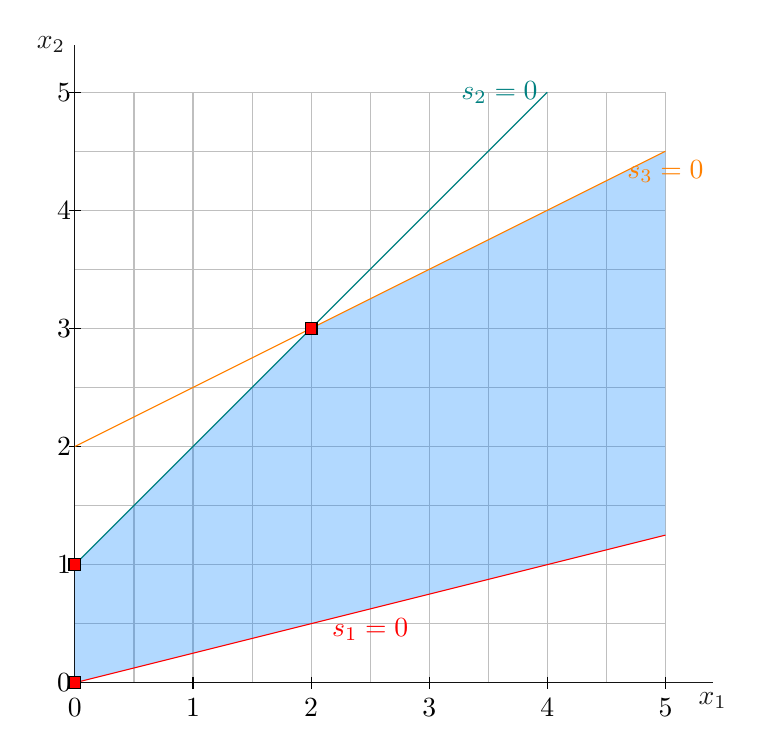
\begin{tikzpicture} [scale=1.5]
    \draw[gray!50, thin, step=.5] (0,0) grid (5,5);
    \draw[opacity=0.9] (0,0) -- (5.4,0) node[below] {$x_1$};
    \draw[opacity=0.9] (0,0) -- (0,5.4) node[left] {$x_2$}; % pilihan \draw[very thick,->]

    \foreach \x in {0,...,5} \draw (\x,0.05) -- (\x,-0.05) node[below] {\x};
    \foreach \y in {0,...,5} \draw (-0.05,\y) -- (0.05,\y) node[left] {\y};

    \fill[blue!50!cyan,opacity=0.3] (0,0) -- (0,1) -- (2,3) -- (5,4.5) --(5,1.25)-- cycle;

    \draw [red](0,0) -- node[below] {$s_1=0$} (5, 1.25);
    \draw [teal] (0,1)  --  (4,5) node[left, sloped] {$s_2=0$};
    \draw [orange](0,2) --  (5,4.5) node[below, sloped] {$s_3=0$}; %node[above right ,sloped]

    \node[fill=blue,circle,inner sep=0.05cm] at (0,0) {};
\node[fill=blue,circle,inner sep=0.05cm] at (0,1) {};
\node[fill=blue,circle,inner sep=0.05cm] at (2,3) {};

\filldraw[fill=red] (-0.05,-0.05) rectangle (0.05,0.05);
\filldraw[fill=red] (-0.05,.95) rectangle (0.05,1.05);
\filldraw[fill=red] (1.95,2.95) rectangle (2.05,3.05);
\end{tikzpicture}\par\captionof{figure}{Daerah layak berbentuk kerucut pada sumbu $x_1$--$x_2$: arsiran biru dibatasi oleh garis $s_1=0$ (merah, bawah), $s_3=0$ (jingga, atas), dan $s_2=0$ (hijau kebiruan, kiri atas); ketiga titik ekstrem ditandai dengan titik biru dan kotak merah.}\label{fig:Section2-tikz11}% fig-num-auto
 \end{center}
\end{minipage}

\begin{center}  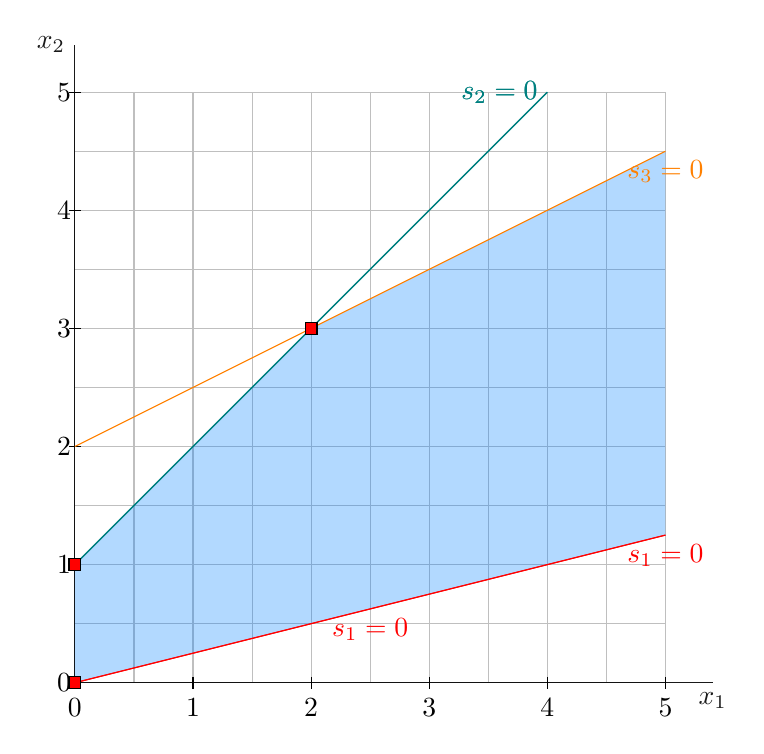
\begin{tikzpicture} [scale=1.5]
    \draw[gray!50, thin, step=.5] (0,0) grid (5,5);
    \draw[opacity=0.9] (0,0) -- (5.4,0) node[below] {$x_1$};
    \draw[opacity=0.9] (0,0) -- (0,5.4) node[left] {$x_2$}; % pilihan \draw[very thick,->]

    \foreach \x in {0,...,5} \draw (\x,0.05) -- (\x,-0.05) node[below] {\x};
    \foreach \y in {0,...,5} \draw (-0.05,\y) -- (0.05,\y) node[left] {\y};

    \fill[blue!50!cyan,opacity=0.3] (0,0) -- (0,1) -- (2,3) -- (5,4.5) --(5,1.25)-- cycle;

\draw[domain=0:4,smooth,variable=\x, teal] plot ({\x},{\x+1}) node[left] {$s_2=0$};
\draw[domain=0:5,smooth,variable=\x, red] plot ({\x},{\x*1/4}) node[below] {$s_1=0$};
\draw [red](0,0) -- node[below] {$s_1=0$} (5, 1.25);
    \draw [teal] (0,1)  --  (4,5) node[left, sloped] {$s_2=0$};
    \draw [orange](0,2) --  (5,4.5) node[below, sloped] {$s_3=0$}; %node[above right ,sloped]
    \node[fill=blue,circle,inner sep=0.05cm] at (0,0) {};
\node[fill=blue,circle,inner sep=0.05cm] at (0,1) {};
\node[fill=blue,circle,inner sep=0.05cm] at (2,3) {};

\filldraw[fill=red] (-0.05,-0.05) rectangle (0.05,0.05);
\filldraw[fill=red] (-0.05,.95) rectangle (0.05,1.05);
\filldraw[fill=red] (1.95,2.95) rectangle (2.05,3.05);
\end{tikzpicture}\par\captionof{figure}{Daerah layak berbentuk kerucut yang sama di antara $s_1=0$ dan $s_3=0$, dengan garis $s_2=0$ di atasnya; daerah diarsir biru, dan titik ekstrem $(0,0)$, $(0,1)$, serta $(2,3)$ ditandai dengan titik biru dan kotak merah.}\label{fig:Section2-tikz12}% fig-num-auto
 \end{center}

%\draw[scale=0.5,domain=-3:3,smooth,variable=\x,blue] plot ({\x},{\x*\x}); % dijadikan komentar karena berada di luar tikzpicture

\medskip Sebagai contoh, perhatikan garis $s_3=0$ (jingga). Untuk mencari arah ekstrem, mulai dari titik ekstrem (2,3), lalu cari titik layak lain pada garis jingga, misalnya (4,4), dan kurangkan (2,3) dari (4,4), sehingga diperoleh (2,1).

\medskip Hal ini berkaitan dengan kemiringan dalam dua dimensi: kenaikannya 1 dan langkah mendatarnya 2. Jadi, arah ini memiliki kemiringan 1/2. Namun, gagasan ini tidak mudah diperluas ke dimensi yang lebih tinggi, tempat arah tidak dapat didefinisikan dengan satu bilangan saja.

\medskip Untuk menemukan arah ekstrem, kita dapat mengubah ruas kanan menjadi $\mathbf{b} = \mathbf{0}$, yang membentuk sebuah kerucut polihedral (berwarna biru-sian), lalu menambahkan kendala $x_1 + x_2 = 1$. Perpotongan kerucut dengan $x_1 + x_2 = 1$ membentuk sebuah ruas garis.

\begin{minipage}[t][][b]{.4\linewidth} \vspace{0mm}
\begin{align*}
\max \quad & z = -5x_1 - x_2  \\
\text{dengan syarat} \quad & x_1 - 4x_2 +s_1 = 0  \\
& -x_1 + x_2 + s_2 = 0 \\
& -x_1 + 2x_2 +s_3 = 0 \\
& x_1 + x_2 = 1 \\
& x_1, x_2, s_1, s_2, s_3 \ge 0.
\end{align*}
\end{minipage}%
\begin{minipage}[t][][b]{.6\linewidth}
\begin{center} 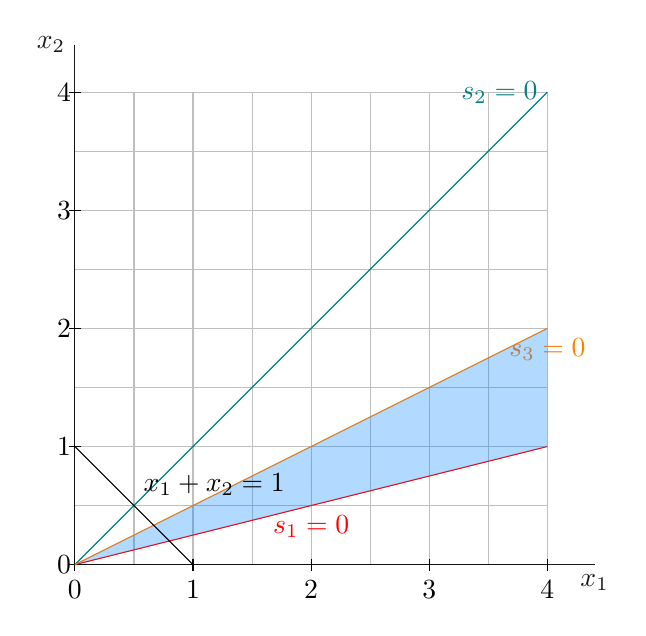
\begin{tikzpicture} [scale=1.5]
\draw[gray!50, thin, step=.5] (0,0) grid (4,4);
\draw[opacity=0.9] (0,0) -- (4.4,0) node[below] {$x_1$};
\draw[opacity=0.9] (0,0) -- (0,4.4) node[left] {$x_2$}; % pilihan \draw[very thick,->]

\foreach \x in {0,...,4} \draw (\x,0.05) -- (\x,-0.05) node[below] {\x};
\foreach \y in {0,...,4} \draw (-0.05,\y) -- (0.05,\y) node[left] {\y};

\draw [red](0, 0) -- node[below] {$s_1=0$} (4, 1);
\draw [teal] (0,0)  -- (4,4) node[left, sloped] {$s_2=0$};
\draw [orange](0,0) -- (4,2) node[below, sloped] {$s_3=0$};
\fill[blue!50!cyan,opacity=0.3] (0,0) -- (4,2) -- (4,1) --  cycle;

\draw [black] (0,1)  -- node[above right] {$x_1+x_2 = 1$} (1,0);
\end{tikzpicture}\par\captionof{figure}{Grafik kerucut resesi: kerucut biru berarsir berada di antara garis $s_1=0$ (merah) dan $s_3=0$ (jingga), sedangkan garis $s_2=0$ (hijau kebiruan) berada di atas kerucut dan garis normalisasi $x_1+x_2=1$ melintasinya.}\label{fig:Section2-tikz13}% fig-num-auto
 \end{center}
\end{minipage}

\Needspace{0.42\textheight}
\begin{center} 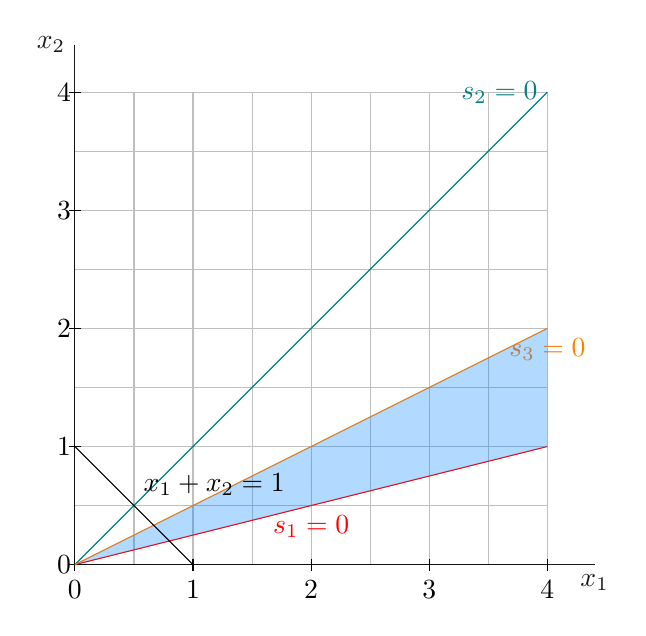
\begin{tikzpicture} [scale=1.5]
\draw[gray!50, thin, step=.5] (0,0) grid (4,4);
\draw[opacity=0.9] (0,0) -- (4.4,0) node[below] {$x_1$};
\draw[opacity=0.9] (0,0) -- (0,4.4) node[left] {$x_2$}; % pilihan \draw[very thick,->]

\foreach \x in {0,...,4} \draw (\x,0.05) -- (\x,-0.05) node[below] {\x};
\foreach \y in {0,...,4} \draw (-0.05,\y) -- (0.05,\y) node[left] {\y};

\draw [red](0, 0) -- node[below] {$s_1=0$} (4, 1);
\draw [teal] (0,0)  -- (4,4) node[left, sloped] {$s_2=0$};
\draw [orange](0,0) -- (4,2) node[below, sloped] {$s_3=0$};
\fill[blue!50!cyan,opacity=0.3] (0,0) -- (4,2) -- (4,1) --  cycle;

\draw [black] (0,1)  -- node[above right] {$x_1+x_2 = 1$} (1,0);
\end{tikzpicture}\par\captionof{figure}{Kerucut resesi yang sama di antara $s_1=0$ dan $s_3=0$, dengan garis $x_1+x_2=1$ yang memotongnya untuk membentuk ruas normalisasi tempat arah ekstrem ditentukan.}\label{fig:Section2-tikz14}% fig-num-auto
 \end{center}

\medskip Untuk memperjelas, kita memperbesar gambar, menghapus garis $s_2=0$ (hijau kebiruan) karena redundan, dan menandai titik-titik ekstrem daerah layak yang baru, (4/5, 1/5) dan (2/3, 1/3), dengan kotak merah. Hasilnya adalah:

\begin{center}  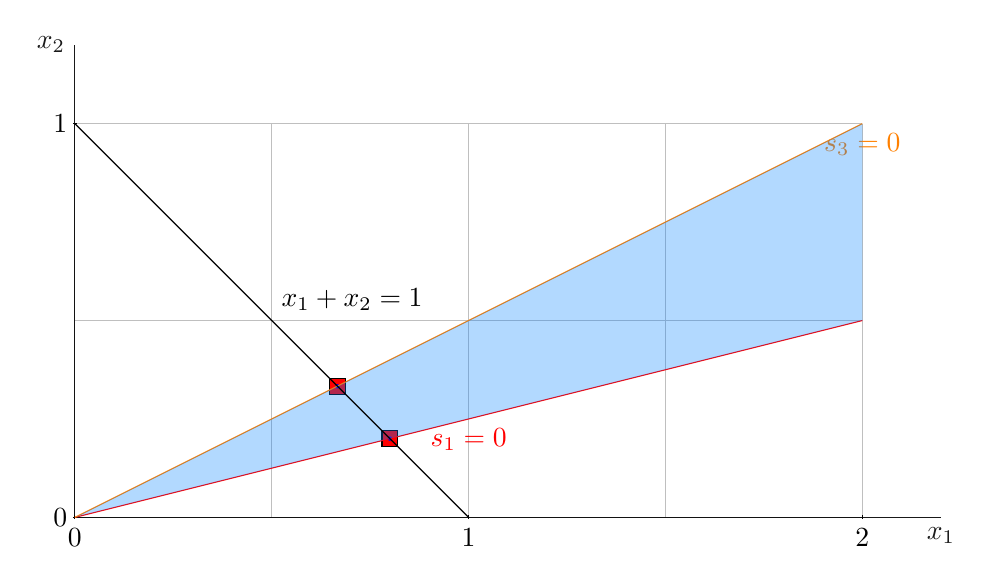
\begin{tikzpicture}[x=50mm, y=50mm]
\draw[gray!50, thin, step=.5] (0,0) grid (2,1);
\draw[opacity=0.9] (0,0) -- (2.2,0) node[below] {$x_1$};
\draw[opacity=0.9] (0,0) -- (0,1.2) node[left] {$x_2$}; % pilihan \draw[very thick,->]

\foreach \x in {0,...,2} \draw (\x,0.005) -- (\x,-0.005) node[below] {\x};
\foreach \y in {0,...,1} \draw (-0.005,\y) -- (0.005,\y) node[left] {\y};

\filldraw[fill=red] (0.8-0.02,0.2-0.02) rectangle (0.8+0.02,0.2+0.02);
\filldraw[fill=red] (0.667-0.02,0.333-0.02) rectangle (0.667+0.02,0.333+0.02);
\node[fill=blue,circle,inner sep=0.02cm] at (0.8,0.2) {};
\node[fill=blue,circle,inner sep=0.02cm] at (0.667,0.333) {};

\draw [red](0, 0) -- node[below] {$s_1=0$} (2, .5);
\draw [orange](0,0) -- (2,1) node[below, sloped] {$s_3=0$};
\fill[blue!50!cyan,opacity=0.3] (0,0) -- (2,.5) -- (2,1) --  cycle;
\draw [black] (0,1)  -- node[above right] {$x_1+x_2 = 1$} (1,0);
\end{tikzpicture}\par\captionof{figure}{Tampilan ruas normalisasi yang diperbesar: garis $x_1+x_2=1$ memotong kerucut berarsir di antara $s_1=0$ dan $s_3=0$ pada titik ekstrem $(4/5,1/5)$ dan $(2/3,1/3)$, yang ditandai dengan titik biru dan kotak merah.}\label{fig:Section2-tikz15}% fig-num-auto
 \end{center}

Jadi, arah ekstremnya adalah (4/5, 1/5) dan (2/3, 1/3). \\
